\newpage
\section{circle 类}

\tkzVar{circle}{C} 变量是一个保留用于存储圆对象的表。虽然它是可选的，任何合法的变量名都可用（例如 \code{Circles}），但强烈建议采用标准名称 \texttt{C}，以保证一致性与可读性。若使用自定义变量，必须手动初始化。\tkzFct{tkz-elements}{init\_elements()} 函数会重置 \texttt{C} 表（如果它已被定义）。


\subsubsection{创建圆}
\label{ssub:creating_a_circle}
圆由两个点定义：
\begin{itemize}
\item 圆心，
\item 圆上一点。
\end{itemize}
\vspace{0.5em}

要创建一个圆，使用如下语法：
\begin{mybox}
\code{C.OA = circle(z.O, z.A)}
\end{mybox}

新创建的圆对象存储各种几何属性，例如半径、直径，以及圆周上的重要点（例如北、东、南、西极点）。

\subsection{圆的属性}

圆对象存储各种几何属性，可访问以作进一步计算或绘图。这些属性在创建时自动计算。

\vspace{1em}

\bgroup
\catcode`_=12
\small
  \captionof{table}{圆的属性。}\label{circle:attributes}
  \begin{tabular}{ll}
  \toprule
  \texttt{属性}         & \texttt{参考}                \\
  \midrule
  \tkzAttr{circle}{type}      &  圆的类型，恒为 "circle"            \\
  \tkzAttr{circle}{center}    &  圆心                       \\
  \tkzAttr{circle}{through}   &  圆所经过的点      \\
  \tkzAttr{circle}{radius}    &  [\ref{ssub:example_circle_attributes}]     \\
  \tkzAttr{circle}{north}     &  [\ref{ssub:example_circle_attributes}]     \\
  \tkzAttr{circle}{south}     &  [\ref{ssub:example_circle_attributes}]     \\
  \tkzAttr{circle}{east}      &  [\ref{ssub:example_circle_attributes}]     \\
  \tkzAttr{circle}{west}      &  [\ref{ssub:example_circle_attributes}]     \\
  \tkzAttr{circle}{opp}       &  [\ref{ssub:example_circle_attributes}]     \\
  \tkzAttr{circle}{ct}        &  [\ref{ssub:example_circle_attributes}]     \\
  \tkzAttr{circle}{perimeter} &  [\ref{ssub:attributes_perimeter_and_area}] \\
  \tkzAttr{circle}{area}      &  [\ref{ssub:attributes_perimeter_and_area}] \\
  \bottomrule %
  \end{tabular}
\egroup



\subsubsection{示例：圆的属性}
\label{ssub:example_circle_attributes}

下面示例展示 \tkzNameObj{circle} 类的若干属性。

\medskip

圆上某给定点的对径点可用下面方法获得：

\begin{center}
\code{z.Mp = C.OA:antipode(z.M)}
\end{center}


用 \code{circle} 创建圆对象时，与定义点（圆所经过的点）对径的点会自动生成并存入属性 \code{opp}。

\medskip

此外，过圆心与该点的直线也会创建，可通过属性 \code{ct}（center-to-through）访问。当处理由函数返回的圆、而你事先不知道用了哪些点构造它时，这一点尤其有用。

\vspace{1em}

\begin{tkzexample}[latex=7cm]
\directlua{
 init_elements()
 z.a = point(1, 1)
 z.b = point(5, 4)
 C.ab = circle(z.a, z.b)
 z.s = C.ab.south
 z.w = C.ab.west
 r = C.ab.radius
 z.c = C.ab.opp
 z.r,
 z.t = C.ab.ct:ortho_from(z.b):get()}
\begin{center}
\begin{tikzpicture}[scale=.5]
  \tkzGetNodes
  \tkzDrawPoints(a,b,c,s,w)
  \tkzLabelPoints(a,b,c,s,w)
  \tkzDrawCircle(a,b)
  \tkzDrawSegments(a,b r,t b,c)
  \tkzLabelSegment[sloped](a,b){ab = \tkzUseLua{r}}
  \end{tikzpicture}
\end{center}
\end{tkzexample}


\subsubsection{属性：周长与面积}
\label{ssub:attributes_perimeter_and_area}

 \pgfkeys{/pgf/number format/.cd,std,precision=4}
 \let\pmpn\pgfmathprintnumber

\begin{mybox}
\begin{verbatim}
  \directlua{
  z.A = point(1, 2)
  z.B = point(4, 3)
  C.AB = circle(z.A, z.B)
  p = C.AB.perimeter
  a = C.AB.area}

设 $A$、$B$ 是两个点。以 $A$ 为圆心且经过 $B$ 的圆，
其周长为 \pmpn{\tkzUseLua{p}} $cm$，
面积为 \pmpn{\tkzUseLua{a} }$cm^2$。
\end{verbatim}
\end{mybox}

\directlua{
z.A = point(1, 2)
z.B = point(4, 3)
C.AB =  circle(z.A, z.B)
p = C.AB.perimeter
a = C.AB.area}

给定两个点 $A$ 与 $B$。
圆心为 $A$、过 $B$ 的圆周长为 \pmpn{\tkzUseLua{p}} $cm$，面积为 \pmpn{\tkzUseLua{a} }$cm^2$。


\newpage
\subsection{circle 类的方法}
circle 类提供大量方法，可按返回值类型分组：数、布尔值、字符串、点、直线或圆。这些方法可用于判断包含、求切线、计算反演等运算。

\vspace{1em}

\bgroup
\catcode`_=12
\small
\captionof{table}{圆的方法。}\label{circle:methods}
\begin{tabular}{ll}
\toprule
\texttt{方法} & \texttt{参考}   \\
\midrule
\texttt{构造函数} & \\
\midrule
\tkzFct{circle}{new(O,A)} & [\ref{ssub:method_circle_new}; \ref{ssub:creating_a_circle}]\\
\tkzFct{circle}{radius(O,r)} & 已弃用；见  [\ref{ssub:method_circle_radius}]\\
\tkzFct{circle}{diameter(A,B)} & 已弃用；见  [\ref{ssub:method_circle_diameter}]\\
\midrule
\texttt{返回实数的方法} & \\
\midrule
\tkzMeth{circle}{power(pt)}& \ref{ssub:power}] \\
\midrule
\texttt{返回字符串的方法} & \\
\midrule
\tkzMeth{circle}{circles\_position(C1)}  & [\ref{ssub:circles_position}] \\
\tkzMeth{circle}{position(obj)} & [\ref{ssub:circle_position}]\\
\tkzMeth{circle}{lines\_position(L)} & [\ref{ssub:method_circle_lines_position}]\\
\midrule
\texttt{返回布尔值的方法} & \\
\midrule
\tkzMeth{circle}{is\_tangent(L)} & [\ref{ssub:method_circle_is_tangent}]  \\
\tkzMeth{circle}{is\_secant(L)} & [\ref{ssub:method_circle_is_secant}]  \\
\tkzMeth{circle}{is\_disjoint(L)} & [\ref{ssub:method_circle_is_disjoint}]  \\
\midrule
\texttt{返回点的方法} & \\
\midrule
\tkzMeth{circle}{get(i)} &     [\ref{ssub:method_circle_get}]   \\
\tkzMeth{circle}{antipode(pt)} & [\ref{ssub:method_circle_antipode}]   \\
\tkzMeth{circle}{midarc(pt,pt)} &  [\ref{ssub:method_circle_midarc}]\\
\tkzMeth{circle}{point(r,<pt>)} & [\ref{ssub:method_circle_point}]\\
\tkzMeth{circle}{random(<'inside'>)}  & [\ref{ssub:method_imeth_circle_random_inside}]\\
\tkzMeth{circle}{inversion(obj)} & [\ref{ssub:inversion}; \ref{par:inversion_circle} \ref{par:inversion_line}]\\
\tkzMeth{circle}{inversion\_neg(obj)} & [\ref{ssub:inversion_neg}]\\
\tkzMeth{circle}{internal\_similitude(C)}  &  [\ref{ssub:method_circle_internal__similitude}]\\
\tkzMeth{circle}{external\_similitude(C)} &  [\ref{ssub:method_circle_external__similitude}] \\
\tkzMeth{circle}{similitude(mode, C)} &  [\ref{ssub:similitude}] \\

\tkzMeth{circle}{radical\_center(C1<,C2>)} & [\ref{ssub:radical_center}]  \\
\tkzMeth{circle}{pole(L)} & [\ref{ssub:method_circle_pole}]\\
\midrule
\texttt{返回直线的方法}  & \\
\midrule
\tkzMeth{circle}{radical\_axis(C)} &   [ \ref{ssub:method_circle_radical__axis_c} ; \ref{par:radical_axis_v1}; \ref{par:radical_axis_v2}; \ref{par:radical_axis_v3}; \ref{par:radical_axis_v4}]  \\
\tkzMeth{circle}{tangent\_at(pt)} &  [\ref{ssub:method_circle_tangent__at_pt}] \\
\tkzMeth{circle}{tangent\_from(pt)}&  [\ref{ssub:method_circle_tangent__from_pt}] \\
\tkzMeth{circle}{tangent\_parallel(L)}&  [\ref{ssub:method_circle_tangent_parallel}] \\
\tkzMeth{circle}{common\_tangent(C)}&  [\ref{ssub:common_tangent}] \\
\tkzMeth{circle}{polar()} & [\ref{ssub:method_circle_polar_pt}] \\
\bottomrule
\end{tabular}
\egroup

\newpage
\bgroup
\catcode`_=12
\small
\captionof{table}{圆的方法}\label{circle:methods 2}
\begin{tabular}{ll}
\toprule
\texttt{返回圆的方法}&\\
\midrule
\tkzMeth{circle}{orthogonal\_from(pt)}  & [\ref{ssub:method_circle_orthogonal_from_pt}]\\
\tkzMeth{circle}{orthogonal\_through(pta,ptb)}&  [\ref{ssub:method_circle_orthogonal_through}]\\
\tkzMeth{circle}{midcircle(C)}  & [\ref{ssub:midcircle}; \ref{midcircle_diameter}] \\
\tkzMeth{circle}{radical\_circle(C1<,C2>)} &  [\ref{ssub:radical_circle}] \\
\tkzMeth{circle}{CPP(pt,pt)} & [\ref{ssub:method_c__c__pp}] \\
\tkzMeth{circle}{CCP(C,pt)} &[\ref{ssub:method_c_cc_p}]  \\
\tkzMeth{circle}{CLP(L,pt,<'inside'>)} & [\ref{ssub:method_c_lc_p}]  \\
\tkzMeth{circle}{CLL}& \ref{ssub:method_c_cll}\\
\tkzMeth{circle}{CCL}(C2, L) & \ref{ssub:CCL}\\
\tkzMeth{circle}{CCC}(C2, C3[, opts]) &  \ref{ssub:CCC}\\
\tkzMeth{circle}{CCC\_gergonne}(C2, C3) &  \ref{ssub:CCC_gergonne}\\
\texttt{返回路径的方法} &     \\
\tkzMeth{circle}{path(pt,pt,nb)} &[\ref{ssub:circle_path}]  \\
\bottomrule
\end{tabular}
\egroup

\bgroup
\catcode`_=12
\small
\captionof{table}{圆构造的辅助函数。}\label{circle:functions}
\begin{tabular}{ll}
\toprule
\texttt{返回两个点的函数} &      \\
\midrule
\tkzFct{circle}{through(pt,r,<angle>)} &  见 [\ref{ssub:function_code_through_and_code_diameter}] \\

\tkzFct{circle}{diameter(pt,pt,<'swap'> or <angle>)}&  见 [\ref{ssub:function_code_through_and_code_diameter}] \\

\bottomrule
\end{tabular}
\egroup



每个方法都可用点语法调用，例如 \code{C.OA:antipode(z.P)} 或 \code{C.OA:radical\_axis(C1)}。已弃用的方法为兼容而保留，但在新代码中应避免使用。

\subsubsection{方法 \tkzMeth{circle}{new}(pt, pt)}
\label{ssub:method_circle_new}

该方法创建一个由两个点定义的新圆对象：
\begin{itemize}
\item 圆的\emph{圆心}，
\item 圆周上的一个\emph{点}，记作 \code{through}。
\end{itemize}
半径按两点间的欧几里得距离计算。在内部，圆对象同时存储圆心与定义点，并计算若干有用属性供进一步几何构造使用。

\vspace{1em}
\texttt{简写： }

函数 \code{circle(center, through)} 等价于 \code{circle:new(center, through)}，为便于使用推荐采用。
\begin{mybox}
\begin{verbatim}
C.OA = circle(z.O, z.A)
-- same as:
C.OA = circle:new(z.O, z.A)
\end{verbatim}
\end{mybox}

\texttt{派生属性： }


创建后，圆对象包含：
\begin{itemize}
\item \code{radius} — 圆心到该点的距离，
\item \code{diameter} — 半径的两倍，
\item \code{opp} — 与 \code{through} 对径的点，
\item \code{ct} — 从圆心到 through 点的有向线段。
\end{itemize}
这些属性自动计算，可用点记法访问（例如 \code{C.OA.radius}、\code{C.OA.opp}）。


\vspace{1em}

\begin{tkzexample}[latex=.5\textwidth]
\directlua{
  init_elements()
  z.O = point(0, 0)
  z.A = point(2, 1)
  C.OA = circle(z.O, z.A)}
\begin{center}
\begin{tikzpicture}[gridded]
 \tkzGetNodes
 \tkzDrawCircle(O,A)
 \tkzDrawPoints(A,O)
 \tkzLabelPoints[right](A,O)
\end{tikzpicture}
  \end{center}
\end{tkzexample}


\subsubsection{函数 \tkzFct{circle}{through} 与 \tkzFct{circle}{diameter}}
\label{ssub:function_code_through_and_code_diameter}

这两个工具函数帮助基于最少数据定义圆。它们本身不返回圆对象，而是返回一对点：\emph{圆心} 与 \emph{圆所经过的点}。这对点可直接传给 \code{circle(...)}，如下所示。

\begin{mybox}
\begin{verbatim}
C.OT = circle(through(z.O, 5))                      -- default angle = 0
C.OT = circle(through(z.O, 5, math.pi / 3))          -- point at 60°
C.OT = circle(diameter(z.A, z.B))                    -- through = B
C.OT = circle(diameter(z.A, z.B, "swap"))            -- through = A
\end{verbatim}
\end{mybox}

\textbf{1. 函数 \code{through(center, radius, <angle>])}}

基于以下要素构造一个圆：
\begin{itemize}
  \item 一个圆心点，
  \item 一个半径（正实数），
  \item 一个可选角（弧度），指定圆周上该点的位置。
\end{itemize}
若省略角度，该点位于从圆心出发的正 \(x\) 轴上（即角度 = 0）。

\textbf{2. 函数 \code{diameter(A, B, <'swap'> or <angle>)}}

用两个对径点构造一个圆。该函数返回：

\begin{itemize}
  \item 以 \([AB]\) 的中点为圆心，
  \item 以两点之一作为 \code{through} 点。
\end{itemize}

默认地，第二个参数（\code{B}）作为 \code{through} 点返回。若给出可选第三个参数 \code{"swap"}，则改用第一个点（\code{A}）。可选角度（弧度）指定圆周上 "through" 点的位置。

\vspace{1em}

\begin{tkzexample}[latex=6cm]
\directlua{
  z.A = point(0, 0)
  z.B = point(2, 1)
  C.T = circle(through(z.A, math.sqrt(5), math.pi / 2))
  C.a = circle(diameter(z.A, z.B))
  z.T = C.T.through
  C.b = circle(diameter(z.A, z.T, "swap"))
  z.w = C.a.center
  z.t = C.a.through
  z.u = C.b.center
  z.v = C.b.through}
\begin{tikzpicture}[gridded]
\tkzGetNodes
 \tkzDrawCircles(A,T w,t u,v)
 \tkzDrawPoints(A,B,T)
 \tkzLabelPoints[right](A,B,T)
\end{tikzpicture}
\end{tkzexample}

\subsubsection{方法 \tkzMeth{circle}{radius(pt,r)}}
\label{ssub:method_circle_radius}

（已弃用，见上文 [\ref{ssub:function_code_through_and_code_diameter}]）

该方法为向后兼容而保留，但不再推荐。它已被更灵活、更面向构造的方式取代。

我们用圆心和半径定义一个圆。

\vspace{1em}
\begin{tkzexample}[latex=.5\textwidth]
\directlua{
  init_elements()
  z.O = point(0, 0)
  z.A = point(2, 1)
  C.T = circle:radius(z.A, math.sqrt(5))
  % better
  % C.T = circle(from_radius(z.A, math.sqrt(5)))
  z.T = C.T.through }
\begin{center}
  \begin{tikzpicture}[gridded]
  \tkzGetNodes
  \tkzDrawCircles(A,T)
  \tkzDrawPoints(A,O,T)
  \tkzLabelPoints[right](A,O,T)
\end{tikzpicture}
\end{center}
\end{tkzexample}


\subsubsection{方法 \tkzMeth{circle}{diameter(pt,pt)}}
\label{ssub:method_circle_diameter}

（已弃用，见上文 [\ref{ssub:function_code_through_and_code_diameter}]）

该方法为向后兼容而保留，但不再推荐。它已被更灵活、更面向构造的方式取代。

圆由其一条直径两端的两个点定义。

\vspace{1em}
\begin{tkzexample}[latex=.5\textwidth]
\directlua{
  init_elements()
  z.A = point(0, 0)
  z.B = point(2, 1)
  C.T = circle:diameter(z.A, z.B)
  % better C.T = from_diameter(z.A, z.B)
  z.O = C.T.center
  z.T = C.T.through}
\begin{center}
\begin{tikzpicture}[gridded]
 \tkzGetNodes
 \tkzDrawCircles(O,T)
 \tkzDrawPoints(A,B,O,T)
 \tkzLabelPoints[right](A,B,O,T)
\end{tikzpicture}
\end{center}
\end{tkzexample}

\subsection{返回布尔值}

\subsubsection{方法 \tkzMeth{circle}{is\_tangent(L)}}
\label{ssub:method_circle_is_tangent}

该方法检查给定直线是否与圆相切。它返回布尔值：直线相切则为 \code{true}，否则为 \code{false}。

\medskip

这在 Lua 中用于逻辑测试与条件构造很有用。该方法利用几何距离与精度容差来判定相切。

\medskip

示例：

\begin{tkzexample}[latex=.5\textwidth]
\directlua{
  z.A = point(0, 0)
  z.B = point(0, 2)
  C.AB = circle(z.A, z.B)
  z.C = point(2, -2)
  z.D = point(2, 3)
  L.CD = line(z.C, z.D)
  if C.AB:is_tangent(L.CD) then
    tex.print("L.CD tangent to C.AB")
  else
    tex.print("L.CD no tangent to C.AB")
  end}
\begin{tikzpicture}
  \tkzGetNodes
  \tkzDrawCircle(A,B)
  \tkzDrawLines(C,D)
  \tkzDrawPoints(A,B,C,D)
  \tkzLabelPoints[below left](A,C)
  \tkzLabelPoints[above right](B,D)
\end{tikzpicture}
\end{tkzexample}

\subsubsection{方法 \tkzMeth{circle}{is\_secant(L)}}
\label{ssub:method_circle_is_secant}
见上面示例

\subsubsection{方法 \tkzMeth{circle}{is\_disjoint(L)}}
\label{ssub:method_circle_is_disjoint}
见上面示例

 \subsubsection{方法 \tkzMeth{circle}{power(pt)}}
 \label{ssub:power}

 \code{power} 方法计算给定点关于给定圆的\emph{点幂}。它定义为：

 \[
 \text{power}(P) = |OP|^2 - r^2
 \]

 其中 $O$ 为圆心，$r$ 为半径。

 \medskip

 结果的符号使我们能判定点 $P$ 的相对位置：
 \begin{itemize}
   \item 正：点在圆外，
   \item 零：点在圆上，
   \item 负：点在圆内。
 \end{itemize}

 \medskip

 下面是一个用函数打印该信息的示例：

 \vspace{1em}
\begin{minipage}{.65\textwidth}
\begin{verbatim}
\directlua{
 init_elements()
 z.O = point(0, 0)
 z.R = point(2, 0)
 z.A = point(1, 1)
 z.B = point(2, -1)
 C.OR = circle(z.O, z.R)
  function position(pt)
 if C.OR:power(pt) > 0
 then
   return tex.print("out")
  else
   return tex.print("in")
 end
  end}
\begin{tikzpicture}
  \tkzGetNodes
  \tkzDrawCircle(O,R)
  \tkzDrawPoints(A,O,B)
  \tkzLabelPoint(A){\tkzUseLua{position(z.A)}}
  \tkzLabelPoint(B){\tkzUseLua{position(z.B)}}
\end{tikzpicture}
\end{verbatim}
 \end{minipage}
 \begin{minipage}{.35\textwidth}
 \directlua{
 init_elements()
 z.O = point(0, 0)
 z.R = point(2, 0)
 z.A = point(1, 1)
 z.B = point(2, -1)
 C.OR = circle(z.O, z.R)
  function position(pt)
 if C.OR:power(pt)>0
 then
 return tex.print("out")
  else
 return tex.print("in")
  end
  end}
\begin{center}
\begin{tikzpicture}
   \tkzGetNodes
   \tkzDrawCircle(O,R)
   \tkzDrawPoints(A,O,B)
   \tkzLabelPoint(A){\tkzUseLua{position(z.A)}}
   \tkzLabelPoint(B){\tkzUseLua{position(z.B)}}
\end{tikzpicture}
\end{center}
\end{minipage}

%--------------------------------------------------------------------
\subsubsection{方法 \tkzMeth{circle}{position(obj)}}
\label{ssub:circle_position}

该方法判定圆与另一对象之间的几何关系。
可提供可选参数 \code{EPS} 来调整数值容差。
默认地，\code{EPS} 为全局值 \tkzVar{tkz}{tkz.epsilon}。

\medskip
\texttt{语法：}

\verb|result = C:position(obj [, EPS])|

\medskip
\texttt{支持的对象类型与返回值}

\begin{itemize}

\item \textbf{点}

返回以下之一：
\begin{itemize}
\item \code{"IN"}  — 点严格在圆盘内，
\item \code{"ON"}  — 点在圆周上，
\item \code{"OUT"} — 点在圆盘外。
\end{itemize}

\item \textbf{直线}

返回以下之一：
\begin{itemize}
\item \code{"DISJOINT"} — 无交点，
\item \code{"TANGENT"}  — 恰有一个公共点，
\item \code{"SECANT"}   — 两个交点。
\end{itemize}

\item \textbf{圆}

返回以下之一：
\begin{itemize}
\item \code{"DISJOINT\_EXT"} — 外离的圆，
\item \code{"TANGENT\_EXT"}  — 外切，
\item \code{"SECANT"}        — 两个交点，
\item \code{"TANGENT\_INT"}  — 内切，
\item \code{"DISJOINT\_INT"} — 一个圆严格在另一个内部，
\item \code{"CONCENTRIC"}    — 同心但半径不同，
\item \code{"COINCIDENT"}    — 两圆重合。
\end{itemize}

\end{itemize}

\medskip
\texttt{注记}

\begin{itemize}
\item 返回值为符号化的大写字符串。
\item 结果带容差判断。
\item 不支持的对象类型会抛出错误。
\end{itemize}

\vspace{1em}

\begin{tkzexample}[latex=.5\textwidth]
\directlua{
  init_elements()
  z.O = point(0, 0)
  z.A = point(1 ,2)
  C.OA = circle(z.O, z.A)
  z.N = point(-2, 2)
  z.M = point(1, 0)
  z.P = point(2, 1)

  PCm = C.OA:position(z.M)
  PDm = C.OA:position_disk(z.M)
  PCn = C.OA:position(z.N)
  PDn = C.OA:position_disk(z.N)
  PCp = C.OA:position(z.P)
  PDp = C.OA:position_disk(z.P)
}

\def\tkzPosPoint#1#2#3#4{%
  \tkzLabelPoints(O,M,N,P)
  \tkzLabelPoint[below=#4pt,
  font=\scriptsize](#2){%
  \tkzUseLua{#1} 位于#3上}%
}

\begin{center}
  \begin{tikzpicture}
  \tkzGetNodes
  \tkzDrawSegments[dashed](O,M O,N O,P)
  \tkzDrawCircle(O,A)
  \tkzDrawPoints(O,M,N,P)

  \tkzPosPoint{PCm}{M}{圆}{8}
  \tkzPosPoint{PCn}{N}{圆}{8}
  \tkzPosPoint{PCp}{P}{圆}{8}

  \tkzPosPoint{PDm}{M}{圆盘}{14}
  \tkzPosPoint{PDn}{N}{圆盘}{14}
  \tkzPosPoint{PDp}{P}{圆盘}{14}
  \end{tikzpicture}
\end{center}
\end{tkzexample}


\subsubsection{方法 \tkzMeth{circle}{in\_out}（用于圆与圆盘）；已弃用}
\label{ssub:in_out_for_circle_and_disk}

以下方法
\code{in\_out()}, \code{in\_out\_disk()},
\code{in\_disk(p)},  \code{in\_out\_disk(p)},
\code{in\_disk\_strict(p)} 与
\code{out\_disk\_strict(p)} 已被 \code{position} 和  \code{position\_disk} 取代。见 [\ref{ssub:circle_position}]

\texttt{注意： } 它们仍然存在，但更推荐使用 \code{position}。

\subsubsection{方法 \tkzMeth{circle}{line\_position(L)}}
\label{ssub:method_circle_line_position}

\texttt{用途： }

该方法对直线相对于圆的位置进行分类。

它返回直线是 \texttt{disjoint}（相离）、\texttt{tangent}（相切）还是 \texttt{secant}（相割）。

\medskip
\texttt{语法： } \verb|pos = C.AB:line_position(L.CD)|

\medskip
\texttt{参数： }

 \texttt{L} — 一个待与圆比较的 \tkzname{line} 对象。

\medskip
\texttt{返回值： }

描述直线相对位置的字符串：
\begin{itemize}
  \item \texttt{"DISJOINT"} — 直线与圆无交点，
  \item \texttt{"TANGENT"} — 直线与圆相切（一个切点），
  \item \texttt{"SECANT"} — 直线与圆交于两点。
\end{itemize}

\medskip
\texttt{注记： }

\begin{itemize}
  \item 半径由圆心与定义点（\texttt{self.through}）计算，
        以保证数值稳定性。
  \item 容差 \tkzVar{tkz}{tkz.epsilon} 用于处理相切附近的舍入误差。
\end{itemize}

\medskip
\texttt{用法示例： }

\begin{tkzexample}[latex=.5\textwidth]
\directlua{
  z.A = point(0, 0)
  z.B = point(4, -2)
  L.AB  = line (z.A, z.B )
  z.O = point(2, 2)
  z.X = z.O + point(0,-2)
  C.OX = circle(z.O, z.X)
  tex.print(C.OX:line_position(L.AB))}
\begin{tikzpicture}[gridded]
 \tkzGetNodes
 \tkzDrawLines[blue](A,B)
 \tkzDrawCircle(O,X)
\end{tikzpicture}
\end{tkzexample}

\subsubsection{方法 \tkzMeth{circle}{lines\_position(L1, L2, mode)}}
\label{ssub:method_circle_lines_position}

\texttt{用途： }

该方法判定圆相对于两条直线的位置。
它根据两直线平行或相割，分析圆触及哪些角域或带域。
结果以整数列表形式返回，对应圆所交的区域。

\texttt{语法： } \verb|sectors = C:lines_position(L1, L2 [, mode])|

\texttt{参数： }

\begin{itemize}
  \item \texttt{L1}, \texttt{L2} — 两个 \tkzname{line} 对象。
  \item \texttt{mode} — 一个可选字符串：
    \begin{itemize}
      \item \texttt{"parallel"} — 若已知两直线平行；
      \item 任何其他值（或省略）—— 默认，用于相割直线。
    \end{itemize}
\end{itemize}

\texttt{返回值： }

一个 Lua 表（整数列表），表示圆所触及区域的编号。

\medskip
对于相割直线：
\begin{itemize}
  \item 区域按逆时针从第一条直线到第二条编号：
        \texttt{1, 2, 3, 4}；
  \item 例如，\texttt{\{1\}} 表示圆完全在第一个区域内，
        而 \texttt{\{4, 1, 2\}} 表示圆触及三个相邻区域。
\end{itemize}

对于平行直线：
\begin{itemize}
  \item 区域编号为：
        \texttt{1} – 两直线之间，
        \texttt{2} – 在 \texttt{L1} 一侧外侧，
        \texttt{3} – 在 \texttt{L2} 一侧外侧；
  \item 示例：
        \texttt{\{1\}} → 圆完全在两直线之间；
        \texttt{\{1,2\}} → 与 \texttt{L1} 相切；
        \texttt{\{1,2,3\}} → 圆足够大，穿过两直线。
\end{itemize}

\texttt{注记： }

\begin{itemize}
  \item 该分类纯几何进行，不计算交点。
  \item 容差 \tkzVar{tkz}{tkz.epsilon} 用于处理相切检测中的数值近似。
\end{itemize}

\texttt{示例（相割直线）}

\begin{tkzexample}[latex=.48\textwidth]
\directlua{
  z.A = point(0, 0)
  z.B = point(3, -2)
  L.AB  = line (z.A, z.B)
  z.C = point(-2, 3)
  z.D = point(3, 1)
  L.CD  = line (z.C, z.D)
  z.O = point(2, 4)
  z.X = z.O + point(0, -1)
  C.OX = circle(z.O, z.X)
  tex.print(C.OX:lines_position(L.AB, L.CD))}
\begin{tikzpicture}
 \tkzGetNodes
 \tkzDrawLines[blue](A,B)
 \tkzDrawLines[red](C,D)
 \tkzDrawCircle(O,X)
 \tkzDrawPoints[red,size=4](A,B,C,D)
 \tkzLabelPoints(A,B,C,D)
\end{tikzpicture}
\end{tkzexample}

\texttt{示例（平行直线）}

\begin{tkzexample}[latex=.48\textwidth]
\directlua{
  z.A = point(0,0)
  z.B = point(4,0)
  L.AB = line(z.A, z.B)
  z.C = point(0,3)
  z.D = point(4,3)
  L.CD = line(z.C, z.D)
  z.O = point(2,1.5)
  z.T = z.O + point(0,1)
  C.OT = circle(z.O, z.T)
  local s = C.OT:lines_position(L.AB,
                    L.CD, "parallel")
  tex.print(s)}
\begin{tikzpicture}
  \tkzGetNodes
  \tkzDrawLines[blue](A,B C,D)
  \tkzDrawCircle(O,T)
\end{tikzpicture}
\end{tkzexample}


%%%%%%%%%%%%%%%%%%%%%%%%%%%%%%%%%%
\subsection{返回实数}
%%%%%%%%%%%%%%%%%%%%%%%%%%%%%%%%%%

\subsubsection{方法 \tkzMeth{circle}{power(pt)}}
\label{ssub:method_circle_power_pt}

点 $A$ 关于半径为~$r$、圆心为~$O$ 的圆的\emph{点幂}是欧几里得几何中的经典概念。

\medskip

它定义为标量：

\[
p = \overline{AP} \cdot \overline{AQ} = AM^2 - r^2
\]

其中：
\begin{itemize}
  \item $P$ 与 $Q$ 为过 $A$ 的直线与圆的交点，
  \item $M$ 为圆心 $O$（故 $AM^2 = |AO|^2$），
  \item 且 $AT$ 为从 $A$ 到圆的切线，满足 $AT^2 = AM^2 - r^2$。
\end{itemize}


几何上：
\begin{itemize}
  \item 若 $A$ 在圆外，点幂为正。
  \item 若 $A$ 在圆上，点幂为零。
  \item 若 $A$ 在圆内，点幂为负。
\end{itemize}

\medskip

在 Lua 中，通过下面的调用求值：

\begin{center}
\code{p = C.XY:power(z.A)}
\end{center}


该值可用于代数计算，或通过其符号判断点的包含关系。

\vspace{1em}

\begin{minipage}{.5\textwidth}
\begin{verbatim}
  \directlua{
  init_elements()
  z.O = point(5, 0)
  z.A = point(0, 0)
  z.R = point(7, 0)
  C.OR = circle(z.O, z.R)
  z.Q = C.OR:point(0.15)
  L.AQ = line(z.A, z.Q)
  _, z.P = intersection(C.OR,L.AQ)
  L.T = C.OR:tangent_from(z.A)
  z.T = L.T.pb}
  \begin{tikzpicture}
  \tkzGetNodes
  \tkzDrawCircle(O,T)
  \tkzDrawPoints(A,O,P,Q,T)
  \tkzDrawSegments(A,O A,Q A,T)
  \tkzLabelPoints(A,O,P,Q,T)
  \tkzText(2,2){$p =\tkzUseLua{%
    C.OR:power(z.A)} =AT^2=AP * AQ$}
  \end{tikzpicture}
\end{verbatim}

\end{minipage}
\begin{minipage}{.5\textwidth}
  \directlua{
  init_elements()
  z.O = point(5,0)
  z.A = point(0,0)
  z.R = point(7,0)
  C.OR = circle(z.O, z.R)
  z.Q = C.OR:point(0.15)
  L.AQ = line(z.A, z.Q)
  _, z.P = intersection(C.OR,L.AQ)
  L.T = C.OR:tangent_from(z.A)
  z.T = L.T.pb}

  \begin{center}
    \begin{tikzpicture}
    \tkzGetNodes
    \tkzDrawCircle(O,T)
    \tkzDrawPoints(A,O,P,Q,T)
    \tkzDrawSegments(A,O A,Q A,T)
    \tkzLabelPoints(A,O,P,Q,T)
    \tkzText(2,2){$p =\tkzUseLua{%
     C.OR:power(z.A)} =AT^2=AP * AQ$}
    \end{tikzpicture}
  \end{center}
\end{minipage}


\subsection{返回字符串}

\subsubsection{方法 \tkzMeth{circle}{circles\_position}}
\label{ssub:circles_position}

该函数返回一个字符串，指示本圆相对于另一圆的位置。便于构造函数。情形为：

\begin{itemize}
   \item \code{outside}
   \item \code{outside tangent}
   \item \code{inside tangent}
   \item \code{inside}
   \item \code{intersect}
\end{itemize}

\begin{minipage}{.55\textwidth}
\begin{verbatim}
\directlua{
init_elements()
   z.A = point(0, 0)
   z.a = point(3, 0)
   z.B = point(2, 0)
   z.b = point(3, 0)
   C.Aa = circle(z.A, z.a)
   C.Bb = circle(z.B, z.b)
   position = C.Aa:circles_position(C.Bb)
   if position == "inside tangent"
   then color = "orange"
   else color = "blue" end}
\begin{tikzpicture}
  \tkzGetNodes
  \tkzDrawCircle(A,a)
  \tkzDrawCircle[color=\tkzUseLua{color}](B,b)
\end{tikzpicture}
\end{verbatim}
\end{minipage}
\begin{minipage}{.45\textwidth}
\directlua{
init_elements()
z.A = point(1, 0)
z.a = point(3, 0)
z.B = point(2, 0)
z.b = point(3, 0)
C.Aa = circle(z.A, z.a)
C.Bb = circle(z.B, z.b)
position = C.Aa:circles_position(C.Bb)
if position == "inside tangent" then color = "orange" else color = "blue" end}


\begin{center}
  \begin{tikzpicture}
  \tkzGetNodes
  \tkzDrawCircle(A,a)
  \tkzDrawCircle[color=\tkzUseLua{color}](B,b)
  \end{tikzpicture}
\end{center}

\end{minipage}


%%%%%%%%%%%%%%%%%%%%%%%%%%%%%%%%%%%%%

%%%%%%  Points %%%%%%%

%%%%%%%%%%%%%%%%%%%%%%%%%%%%%%%%%%%%%

\subsection{返回点}

\subsubsection{方法 \tkzMeth{circle}{get()}}
\label{ssub:method_circle_get}

该方法取出圆的定义点。
圆由其圆心及圆周上一点确定。

\begin{itemize}
  \item \code{C:get()} 返回圆心及圆所经过的一点。
  \item \code{C:get(1)} 返回圆心。
  \item \code{C:get(2)} 返回圆周上的点。
\end{itemize}

当需要复用圆的几何定义时该方法很有用，例如构造切线、根轴，或把圆的数据传给其他构造时。
它提供一种简单而一致的方式来访问定义圆的基本点。



\subsubsection{方法 \tkzMeth{circle}{antipode}}
\label{ssub:method_circle_antipode}
该方法用于定义与给定圆上某点对径的点。

\vspace{1em}
\begin{tkzexample}[latex=.5\textwidth]
\directlua{
  init_elements()
  z.A = point(0, 0)
  z.O = point(2, 1)
  C.OA = circle(z.O, z.A)
  z.B = C.OA:antipode(z.A)}
\begin{center}
\begin{tikzpicture}[gridded]
  \tkzGetNodes
  \tkzDrawCircles(O,A)
  \tkzDrawPoints(A,B,O)
  \tkzLabelPoints[right](A,B,O)
\end{tikzpicture}
\end{center}
\end{tkzexample}

\subsubsection{方法 \tkzMeth{circle}{midarc}}
\label{ssub:method_circle_midarc}

经典定义见 \href{https://mathworld.wolfram.com/Mid-ArcPoints.html}{MathWorld}，如下：

\medskip
\begin{quote}
三角形的弧中点（mid-arc points），按 Johnson（1929）的定义，是三角形外接圆上位于由三角形顶点所确定的三段弧各自中点的点。这些点出现在富尔曼圆（Fuhrmann circle）与富尔曼三角形（Fuhrmann triangle）的定义中，它们位于从外心作出的三角形各边垂直平分线的延长线上。
\end{quote}

\medskip

在本文语境中，该定义被推广。该方法返回圆上把给定弧按角度度量等分的点。换言之，它计算由圆上两点所定义弧的（角度）中点。

\medskip

该方法适用于圆上任意一对点，而不仅限于与三角形顶点或外接圆相关的点。

\vspace{1em}
\begin{tkzexample}[latex=.5\textwidth]
\directlua{
  init_elements()
  z.A = point(0, 0)
  z.O = point(2, 1)
  C.OA = circle(z.O, z.A)
  z.B = C.OA:point(0.25)
  z.M = C.OA:midarc(z.A, z.B)}
\begin{center}
\begin{tikzpicture}[gridded]
  \tkzGetNodes
  \tkzDrawCircles(O,A)
  \tkzDrawPoints(A,B,O,M)
  \tkzLabelPoints[right](A,B,O,M)
\end{tikzpicture}
  \end{center}
\end{tkzexample}

\subsubsection{方法 \tkzMeth{circle}{point(r,<pt>)}}
\label{ssub:method_circle_point}

设 $C$ 为以 $O$ 为圆心、过 $A$ 的圆，其中 $z.A = C.through$。

该方法在圆上定义一点 $M$，使弧长与圆周长之比等于 $r$。

默认地，弧从参考点 $A$ 起量。
可选参数 \texttt{pt} 允许用户指定圆上另一起点。

因此，若给出 \texttt{pt}，则点 $M$ 定义为使弧 $\widearc{(\texttt{pt})M}$ 的长度与圆周长之比等于 $r$。

在下例中，$r=\dfrac{1}{6}$ 对应 $\dfrac{\pi/3}{2\pi}$，故角 $\widehat{AOB}$ 的度量为 $\pi/3$。

若 $r=0.5$，所定义的点与参考点对径。

\vspace{1em}
\begin{tkzexample}[latex=.5\textwidth]
\directlua{
 init_elements()
 z.O = point(0, 0)
 z.A = point(1, 2)
 z.E = point(-1, 2)
 C.OA = circle(z.O, z.A)
 z.B = C.OA:point(1 / 6)
 % from A (default)
 z.C = C.OA:point(0.25)
 z.D = C.OA:point(0.5)
 z.F = C.OA:point(1 / 6, z.E)
 % from E (custom origin)
}
\begin{center}
\begin{tikzpicture}
\tkzGetNodes
\tkzDrawCircle(O,A)
\tkzDrawPoints(A,...,F,O)
\tkzLabelPoints(A,...,F,O)
\end{tikzpicture}
\end{center}
\end{tkzexample}



\subsubsection{方法 \tkzMeth{circle}{random(<'inside'>)}}
\label{ssub:method_imeth_circle_random_inside}
产生圆上一点；若使用 'inside' 选项，则在圆盘内部产生一点。


\begin{minipage}{.5\textwidth}
\directlua{
  init_elements()
  z.O = point(0, 2)
  z.A = point(2, 1)
  C.OA = circle(z.O, z.A)
  z.M = C.OA:random()
  z.N = C.OA:random('inside')}
\begin{center}
\begin{tikzpicture}
   \tkzGetNodes
   \tkzDrawCircle(O,A)
   \tkzDrawPoints(O,A,M,N)
   \tkzLabelPoints(O,A,M,N)
\end{tikzpicture}
\end{center}
\end{minipage}
\begin{minipage}{.5\textwidth}
\begin{tkzexample}[code only]
\directlua{
  init_elements()
  z.O = point(0, 2)
  z.A = point(2, 1)
  C.OA = circle(z.O, z.A)
  z.M = C.OA:random()
  z.N = C.OA:random('inside')}
\end{tkzexample}
\end{minipage}

\subsubsection{方法 \tkzMeth{circle}{internal\_similitude(C)}}
\label{ssub:method_circle_internal__similitude}

此方法计算两个给定圆的\textbf{内相似中心}。

\medskip

两个圆（一般位置下）总是存在两个位似中心：
\begin{itemize}
  \item \textbf{内相似中心}，位于两圆心之间，并按半径之比内分连接两圆心的线段，
  \item \textbf{外相似中心}，位于线段之外，并按同样的比外分该线段。
\end{itemize}


这些中心位于连接两圆心的直线上，该直线称为\emph{连心线}。

\medskip

此方法返回内位似中心——从该点看两个圆方向相同、比例一致，仿佛一个圆在内部缩放为另一个圆。

\medskip

\emph{注：}退化情形（例如圆心相同、半径相等或为零）单独处理。
\begin{flushright}
\small
\href{https://en.wikipedia.org/wiki/Homothetic_center}{\textit{(See also: Wikipedia — Homothetic center)}}
\end{flushright}

\vspace{1em}


\begin{tkzexample}[latex=.5\textwidth]
\directlua{
  init_elements()
  z.A = point(0, 0)
  z.a = point(2, 2)
  z.B = point(5 , 2)
  z.b = point(6 , 1)
  C.Aa = circle(z.A, z.a)
  C.Bb = circle(z.B, z.b)
  z.I = C.Aa:internal_similitude(C.Bb)
  L.TA1, L.TA2 = C.Aa:tangent_from(z.I)
  z.A1 = L.TA1.pb
  z.A2 = L.TA2.pb}
 \begin{center}
 \begin{tikzpicture}[ scale =.6]
   \tkzGetNodes
   \tkzDrawCircles(A,a B,b)
  \tkzDrawPoints(A,a,B,b,I,A1,A2)
  \tkzDrawLines[add = 1 and 2](A1,I A2,I)
 \end{tikzpicture}
 \end{center}
\end{tkzexample}

\subsubsection{方法 \tkzMeth{circle}{external\_similitude(C)}}
\label{ssub:method_circle_external__similitude}


此方法计算两个给定圆的\textbf{外相似中心}。

\medskip

与内相似中心的情况一样，一般位置下的两个圆有两个位似中心。外相似中心位于\emph{连心线}上，但在连接两圆心的线段之外。

\medskip

它按两圆半径之比\emph{外分}这条直线。该中心是唯一的、从它看两个圆互为反向缩放像的点。

\medskip

这种构造在许多几何变换（例如反演、相似、共轴系）以及中间圆和阿波罗尼奥斯圆理论中都很重要。

\medskip

\emph{注：}与内相似中心一样，圆心相同或半径为零等退化情形单独处理。

\vspace{1em}

\begin{tkzexample}[latex=.5\textwidth]
\directlua{
  init_elements()
  z.A = point (0 , 0 )
  z.a = point (2 , 2)
  z.B = point (3 , 2 )
  z.b = point(3.5, 1 )
  C.Aa = circle(z.A, z.a)
  C.Bb = circle(z.B, z.b)
  z.I = C.Aa:external_similitude(C.Bb)
  L.TA1,L.TA2 = C.Aa:tangent_from(z.I)
  z.A1 = L.TA1.pb
  z.A2 = L.TA2.pb}
\begin{center}
\begin{tikzpicture}[scale = .75]
\tkzGetNodes
\tkzDrawCircles(A,a B,b)
\tkzDrawPoints(A,a,B,b,I,A1,A2)
\tkzDrawLines[add = .25 and .1](A1,I A2,I)
\end{tikzpicture}
\end{center}
\end{tkzexample}

\subsubsection{方法 \tkzMeth{circle}{similitude(C,mode)}}
\label{ssub:similitude}

此方法统一了两个相似中心函数。

\begin{itemize}
  \item \code{mode = "internal"} 返回内相似中心。
  \item \code{mode = "external"} 返回外相似中心。
\end{itemize}

\medskip
\noindent\texttt{Example: }
\begin{verbatim}
S  = C1:similitude(C2, "internal")
Se = C1:similitude(C2, "external")
\end{verbatim}


\subsubsection{方法 \tkzMeth{circle}{radical\_center(C1, C2)}}
\label{ssub:radical_center}

在经典几何中，三个圆的\textbf{根心}（也称为\emph{幂心}）是它们的根轴两两相交的唯一交点。

\medskip

这一基本结果归功于 Gaspard Monge（参见 Dörrie 1965，第 153 页），它指出：
\begin{quote}
任意三个圆（其中任意两个圆心不同）的根轴相交于一点——即根心。
\end{quote}


（另见：\href{[URL1]}{MathWorld — Radical Center}）

\medskip

在本实现中，方法 \code{radical\_center(C1, C2)} 在仅应用于两个圆时也有
明确的意义。
返回的点
\[
\code{z.P = C1:radical\_center(C2)}
\]
是两圆的\emph{根轴}与直线的交点，
该直线连接两圆的圆心。

这个点可以看作是\emph{推广的根心}。
它是与两个给定圆都正交的一个特殊圆的圆心。
这个圆属于与 \code{C1} 和 \code{C2} 正交的共轴圆束；
它与连心线的交点
与这个圆束的两个固定基点重合。

这种构造自然推广到圆与点的情况。
点 $P$ 被解释为\emph{圆点}，即半径为
零的圆：
\[
\code{z.P = point(a,b)}, \qquad \code{C.P = circle(z.P,z.P)}.
\]
在这种情况下，根心是唯一与给定圆正交且
过点 $P$ 的圆的圆心。


\medskip

这个点在涉及反演、共轴系以及阿波罗尼奥斯圆等特殊构形的构造中很有用。

\texttt{示例：三个圆、两个圆、一个圆以及一个点}

\begin{tkzexample}[vbox]
\directlua{
 z.A = point(0, 0)
 z.a = z.A + point (1, 0)
 z.B = point (4, 1)
 z.b = z.B + point (2, 0)
 z.C = point (2, 6)
 z.c = z.C + point (3, 0)
 C.Aa = circle(z.A, z.a)
 C.Bb = circle(z.B, z.b)
 C.Cc = circle(z.C, z.c)
 L.rAB = C.Aa:radical_axis(C.Bb)
 L.rAC = C.Aa:radical_axis(C.Cc)
 L.rBC = C.Bb:radical_axis(C.Cc)
 z.w = C.Aa:radical_center(C.Bb, C.Cc)
 z.x1, z.y1 = L.rAB:get()
 z.x2, z.y2 = L.rAC:get()
 z.x3, z.y3 = L.rBC:get()
 z.t = C.Aa:radical_circle(C.Bb, C.Cc).through
 z.w1, z.t1 = C.Aa:radical_circle(C.Bb):get()
 C.B = circle(z.B, z.B)
 z.w2, z.t2 = C.Aa:radical_circle(C.B):get()}
\begin{center}
\begin{tikzpicture}
   \tkzGetNodes
   \tkzDrawCircles[blue](A,a B,b C,c)
   \tkzDrawCircles[red](w,t)
   \tkzDrawCircles[orange](w1,t1)
   \tkzDrawCircles[purple](w2,t2)
   \tkzDrawLines[red](x1,y1 x2,y2 x3,y3)
   \tkzDrawPoints(A,B,C,w,w1,w2)
   \tkzLabelPoints[below right](A,B,C,w,w1,w2)
\end{tikzpicture}
\end{center}
\end{tkzexample}


\subsubsection{方法 \tkzMeth{circle}{pole(L)}}
\label{ssub:method_circle_pole}

\texttt{Syntax:}
\begin{verbatim}
P = circle:pole(L)
\end{verbatim}

\texttt{Purpose:}
计算直线 \(L\) 关于当前圆的\emph{极点}。
极点就是极线恰为直线 \(L\) 的点。

\medskip
\texttt{Arguments:}
\begin{itemize}
  \item \code{L} —— 一个 line 对象。
\end{itemize}

\medskip
\texttt{Returns:}
\begin{itemize}
  \item 点 \(P\)，使得 \(P\) 关于该圆的极线为 \(L\)；
  \item 若直线过圆心，则返回 \code{nil,"INFINITE"}。
\end{itemize}

\medskip
\texttt{Geometric principle:}
设 \(O\) 为圆心，\(R\) 为半径。
用 \(H\) 表示 \(O\) 在直线 \(L\) 上的正交投影。
若 \(H \neq O\)，则 \(H\) 关于该圆的反演点，
满足 \(OH \cdot OP = R^2\)，
即为直线 \(L\) 的极点 \(P\)。

\[
P = \mathrm{Inv}_{(O,R)}(H),
\qquad \text{with } H = \mathrm{proj}_L(O)
\]

若 \(H = O\)（即直线过圆心），
极点是在过 \(O\) 垂直于 \(L\) 的直线上的\emph{无穷远点}。



\medskip
\texttt{Example:}

\directlua{
 init_elements()
 z.A = point(0, 0)
 z.B  = point(-1, 2)
 C.AB = circle(z.A, z.B)
 z.C =  point(0, -4)
 z.D =  point(5, 0)
 L.CD = line(z.C, z.D)
 z.P = C.AB:pole(L.CD)}
\begin{center}
 \begin{tikzpicture}
\tkzGetNodes
\tkzDrawCircles(A,B)
\tkzDrawLines(C,D)
\tkzDrawPoints(A,...,D,P)
\tkzLabelPoints(A,...,D,P)
\end{tikzpicture}
 \end{center}
%%%%%%%%%%%%%%%%%%%%%%%%%%%%%%%%%%%%%

%%%%%%  Lines %%%%%%%

%%%%%%%%%%%%%%%%%%%%%%%%%%%%%%%%%%%%%

\subsection{Returns a line}

\subsubsection{方法 \tkzMeth{circle}{tangent\_at(pt)}}
\label{ssub:method_circle_tangent__at_pt}

此方法构造圆在其圆周上给定点处的切线。

\medskip

结果是以切点为中心的直线段。其两个端点关于切点对称放置、与切点等距，便于绘制和标注。

\medskip

在下面的示例中，点 \code{Tx} 和 \code{Ty} 是切点处切线段的两端点。

\medskip

此方法可用于在图形中突出相切关系、构造切线方向或定义正交投影。

\vspace{1em}


\begin{minipage}{.5\textwidth}
\directlua{
 init_elements()
 z.A = point(0,0)
 z.B = point(1,2)
 C.AB = circle(z.A, z.B)
 L.T = C.AB:tangent_at(z.B)
 z.Tx, z.Ty = L.T:get()}
\begin{tikzpicture}
\tkzGetNodes
\tkzDrawCircle(A,B)
\tkzDrawLines[add =.25 and .25](Tx,Ty)
\tkzDrawSegments[dashed](A,B)
\tkzDrawPoints(A,B)
\tkzLabelPoints[below left](A)
\tkzLabelPoints[above right](B)
\tkzMarkRightAngles(A,B,Tx)
\end{tikzpicture}
\end{minipage}
\begin{minipage}{.5\textwidth}
\begin{tkzexample}[code only]
\directlua{
 init_elements()
 z.A = point(0,0)
 z.B = point(1,2)
 C.AB = circle(z.A, z.B)
 L.T = C.AB:tangent_at(z.B)
 z.Tx, z.Ty = L.T:get()}
\end{tkzexample}
\end{minipage}

\subsubsection{方法 \tkzMeth{circle}{tangent\_from(pt)}}
\label{ssub:method_circle_tangent__from_pt}

此方法计算自圆外一点引出的两条切线。

\medskip

给定位于圆外的点 $P$，过 $P$ 且与圆相切的直线恰有两条。此方法返回这两条切线，每条由 $P$ 和与圆的切点确定。

\medskip

切点也可作为这些直线的端点访问。它们是切线与圆相切的唯一位置，且与半径正交。

\medskip

这种构造在许多经典几何构形中很有用（根轴、三角形内切圆的切线等）。

\vspace{1em}


\begin{minipage}{.5\textwidth}
\directlua{
 init_elements()
 z.A = point(0,0)
 z.B = point(1,2)
 C.AB = circle(z.A, z.B)
 z.C = point(3,-2)
 L.T1,L.T2 = C.AB:tangent_from(z.C)
 z.T1 = L.T1.pb
 z.T2 = L.T2.pb}
\begin{center}
  \begin{tikzpicture}
  \tkzGetNodes
  \tkzDrawCircle(A,B)
  \tkzDrawLines[add =.5 and .5](C,T1 C,T2)
  \tkzDrawSegments[dashed](A,T1 A,T2)
  \tkzDrawPoints(A,...,C,T1,T2)
  \tkzLabelPoints[below left](A,T2,C)
  \tkzLabelPoints[above right](B,T1)
  \tkzMarkRightAngles(A,T1,C A,T2,C)
  \end{tikzpicture}
\end{center}

\end{minipage}
\begin{minipage}{.5\textwidth}
\begin{tkzexample}[code only]
\directlua{
 init_elements()
 z.A = point(0,0)
 z.B = point(1,2)
 C.AB = circle(z.A, z.B)
 z.C = point(3,-2)
 L.T1,L.T2 = C.AB:tangent_from(z.C)
 z.T1 = L.T1.pb
 z.T2 = L.T2.pb}
\end{tkzexample}
\end{minipage}

\subsubsection{方法 \tkzMeth{circle}{tangent\_parallel(line)}}
\label{ssub:method_circle_tangent_parallel}
此方法构造与给定方向（以一条直线给出）\emph{平行}的圆的两条切线。
\medskip

每条切线返回为以其与圆的切点为中心的直线段。为便于绘制和标注，每条切线段的两端点关于切点对称放置、与切点等距。
\medskip


\begin{verbatim}
 L1, L2 = C:tangent_parallel(Ldir)
\end{verbatim}

\begin{tkzexample}[latex = .5\textwidth]
\directlua{
 init_elements()
 z.A = point(0, 0)
 z.B = point(4, 4)
 L.AB = line(z.A, z.B)
 z.O = point(3, -2)
 z.T = point(3, 0)
 C.OT = circle(z.O, z.T)
 L.T1, L.T2 = C.OT:tangent_parallel(L.AB)
 z.x, z.y = L.T1:get()
 z.u, z.v = L.T2:get()
 z.M = L.T1.mid
 z.N = L.T2.mid}
\begin{center}
\begin{tikzpicture}[scale=.5]
\tkzGetNodes
\tkzDrawCircle(O,T)
\tkzDrawLines(A,B x,y u,v)
\tkzDrawPoints(O,A,B,M,N)
\tkzLabelPoints(O,A,B,M,N)
\end{tikzpicture}
\end{center}
\end{tkzexample}


\subsubsection{方法 \tkzMeth{circle}{common\_tangent(C)}}
\label{ssub:common_tangent}

此方法构造两圆的\textbf{公切线}。
它支持 \verb|mode| 的三种选项：
\verb|"external"|（默认）、\verb|"internal"| 和 \verb|"both"|。
此方法以直线的形式返回切线：一般情况下两条，当两圆
相切时一条（切点处的切线），使用 \verb|"both"| 时最多四条
（外切线在前）。如果所请求类别的切线不存在，则
抛出错误。
解的数量取决于两圆的相对位置，范围为 0 到 4。
\medskip

典型情形：
\begin{itemize}
\small
\item \textbf{相离（分离）的圆：} 4 条切线（2 条外公切线，2 条内公切线）。
\item \textbf{外切的圆（相切于一点）：} 3 条切线（2 条外公切线，1 条内公切线）。
\item \textbf{相交的圆（两个交点）：} 2 条切线（均为外公切线）。
\item \textbf{内切的圆（一个在另一个内部并相切）：} 1 条切线（外公切线）。
\item \textbf{一个圆严格包含在另一个圆内（无接触）：} 0 条切线。
\end{itemize}

注意事项与约定：
\begin{itemize}
\item \verb|mode="external"| 返回外公切线；\verb|mode="internal"| 返回内公切线。
\item 退化情形已明确处理：重合的圆有无限多条公切线（未定义），半径不同的同心圆没有任何公切线。
\item 当半径相等且两圆相离时，仍有 4 条切线；外位似中心在无穷远处，这可能影响构造方法，但不影响结果。
\end{itemize}

\medskip


\begin{tkzexample}[latex=.45\textwidth]
\directlua{
 init_elements()
 z.A = point(0, 0)
 z.a = point(4, 0)
 z.B = point(6, 0)
 z.b = point(5, 0)
 C.Aa = circle(z.A, z.a)
 C.Bb = circle(z.B, z.b)
 L.Tx, L.Ty = C.Aa:
    common_tangent(C.Bb,"external")
 z.x, z.y = L.Tx:get()
 z.xp, z.yp = L.Ty:get()
 L.Tu, L.Tv = C.Aa:
    common_tangent(C.Bb,"internal")
 z.u, z.v = L.Tu:get()
 z.up, z.vp = L.Tv:get()}
\begin{center}
\begin{tikzpicture}[scale =.5]
  \tkzGetNodes
  \tkzDrawCircles(A,a B,b)
  \tkzDrawLines[red](x,y x',y' u,v u',v')
  \tkzDrawPoints(x,y,x',y',u,v,u',v')
\end{tikzpicture}
\end{center}
\end{tkzexample}


\texttt{Application: }
\medskip

设 $T$ 和 $T'$ 是两圆的一条外公切线的切点，选择方式使 $T$ 位于第一个圆上、$T'$ 位于第二个圆上，且都在同侧。考虑一条过定点 $C$（通常是其中一个圆的圆心）且平行于该切线的割线。

\medskip

在此构形中，线段 $[TT']$ 从割线与第二个圆的另一交点 $D$ 看，所张的角等于\emph{两给定圆夹角的一半}。

\medskip

这个优美的几何关系用于构造与两圆相关的切线和角平分线。

\vspace{1em}


\begin{minipage}{.55\textwidth}
\directlua{
init_elements()
z.A = point(0 , 0 )
z.B = point(5 , 2 )
L.AB = line(z.A, z.B)
z.C = point(1, 2)
C.AC = circle(z.A, z.C)
C.BC = circle(z.B, z.C)
L.TTp = C.AC:common_tangent(C.BC)
z.T, z.Tp = L.TTp:get()
z.M = C.AC:point(0.45)
L.MC =line(z.M, z.C)
z.Mp = intersection(L.MC, C.BC)
L.mm = L.TTp:ll_from(z.C)
_, z.M = intersection(L.mm, C.AC)
z.Mp = intersection(L.mm, C.BC)
_, z.D = intersection(C.AC,C.BC)}
\begin{center}
  \begin{tikzpicture}[scale =.75]
  \tkzGetNodes
  \tkzDrawCircles(A,C B,C)
  \tkzDrawSegments(M,M' A,D B,D A,B C,D
    T,C T',C)
  \tkzDrawSegments[gray](D,M D,M' T,T'
    D,T D,T')
  \tkzDrawPoints(A,B,C,D,M,M',T,T')
  \tkzLabelPoints(A,B,D,M)
  \tkzLabelPoints[above](C,M',T,T')
  \tkzMarkAngles[mark=|,size=.75](T,C,M C,T,T'
       C,D,T T,D,M)
  \tkzMarkAngles[mark=||,size=.75](M',C,T'
  T,T',C T',D,C M',D,T')
\end{tikzpicture}
\end{center}
\end{minipage}
\begin{minipage}{.4\textwidth}
\begin{tkzexample}[code only]
\directlua{
init_elements()
z.A = point(0 , 0 )
z.B = point(5 , 2 )
L.AB = line(z.A, z.B)
z.C = point(1, 2)
C.AC = circle(z.A, z.C)
C.BC = circle(z.B, z.C)
L.TTp = C.AC:common_tangent(C.BC)
z.T, z.Tp = L.TTp:get()
z.M = C.AC:point(0.45)
L.MC =line(z.M, z.C)
z.Mp = intersection(L.MC, C.BC)
L.mm = L.TTp:ll_from(z.C)
_, z.M = intersection(L.mm, C.AC)
z.Mp = intersection(L.mm, C.BC)
_, z.D = intersection(C.AC,C.BC)}
\end{tkzexample}
\end{minipage}

\subsubsection{方法 \tkzMeth{circle}{polar(pt)}}
\label{ssub:method_circle_polar_pt}

在射影几何中，\emph{极点}与\emph{极线}的概念给出了点与直线关于圆锥曲线的对偶关系。

\medskip

在圆的特殊情形下，这种对偶关系变得尤为优美。方法 \code{polar(pt)} 计算给定点关于该圆的\textbf{极线}。

\medskip

这种构造基于圆内的\textbf{反演}：
\begin{itemize}
  \item 点 $Q$（不在圆心）的\textbf{极线}定义为过 $Q$ 关于该圆的\emph{反演点}、且垂直于过 $Q$ 的半径的直线。
  \item 反之，直线 $L$（不过圆心）的\textbf{极点}是圆心到该直线垂足（关于该圆）的反演点。
\end{itemize}


此方法目前仅支持以\emph{点}为参数的情形。结果是直线——该点的极线。

\medskip

（另见：\href{[URL1]}{Wikipedia — Pole and polar}）

\vspace{1em}


\begin{tkzexample}[latex = .5\textwidth]
\directlua{
 init_elements()
 z.o = point(-1,1)
 z.t = point(1,3)
 z.P = point(3.2,0)
 C.o = circle(z.o, z.t)
 L.P = C.o:polar(z.P)
 z.a, z.b = L.P:get()
 z.u, z.v = intersection(C.o,L.P)
 z.K = L.P:projection(z.P)
 L.K = C.o:polar(z.K)
 z.ka, z.kb = L.K:get()
 C.wH = C.o:inversion(L.P)
 z.w, z.H = C.wH:get()
 z.ap, z.bp = C.o:inversion(z.a, z.b)
 L.oa = line(z.o, z.a)
 z.cp = intersection(L.K,L.oa)
 z.c = C.o:inversion(z.cp)}
\begin{center}
\begin{tikzpicture}
  \tkzGetNodes
  \tkzDrawCircles[red,thick](o,t)
  \tkzDrawCircles(w,H)
  \tkzDrawLines[red](P,u P,v)
  \tkzDrawLines[blue,thick](u,v)
  \tkzDrawLines[add = 1 and 1,
     green!50!black,thick](ka,kb)
  \tkzDrawSegments[dashed](o,P o,c' o,b' K,c)
  \tkzMarkRightAngle[size=.1,
     fill=lightgray!15](o,c,K)
  \tkzDrawPoints(o,w,K,P,a,b,u,v,a',b',c',c)
  \tkzLabelPoints(o,w,b')
  \tkzLabelPoints[above right,blue](a,b,u,v)
  \tkzLabelPoints[above](c,a',c')
  \tkzLabelPoints[right,blue](P)
  \tkzLabelPoints[green!50!black,left](K)
 \end{tikzpicture}
\end{center}
\end{tkzexample}

\subsubsection{方法 \tkzMeth{circle}{radical\_axis}(C)}
\label{ssub:method_circle_radical__axis_c}

根直线（也称根轴）是相对于两个非同心圆具有相等圆幂的点的轨迹。由弦定理可知，它垂直于连心线（Dörrie 1965）。
\begin{flushright}
\small
 \href{[URL1]}{Weisstein, Eric W. "Radical Line." From MathWorld--A Wolfram Web Resource.}
\end{flushright}

\vspace{1em}
根轴 v1
\label{par:radical_axis_v1}

\vspace{1em}

\begin{minipage}{.5\textwidth}
\directlua{
 init_elements()
 z.X = point(0,0)
 z.B = point(2,2)
 z.Y = point(7,1)
 z.Ap = point(8,-1)
 L.XY = line(z.X, z.Y)
 C.XB = circle(z.X, z.B)
 C.YAp = circle(z.Y, z.Ap)
 z.E, z.F = C.XB:radical_axis(C.YAp):get()
 z.A = C.XB:point(0.4)
 T.ABAp = triangle(z.A, z.B, z.Ap)
 z.O = T.ABAp.circumcenter
 C.OAp = circle(z.O, z.Ap)
 _, z.Bp = intersection(C.OAp,C.YAp)
 L.AB = line(z.A, z.B)
 L.ApBp = line(z.Ap, z.Bp)
 z.M = intersection(L.AB,L.ApBp)
 z.H = L.XY:projection(z.M)}
 \begin{center}
   \begin{tikzpicture}[scale = .4]
   \tkzGetNodes
   \tkzDrawCircles(X,B Y,A')
   \tkzDrawArc[dashed,delta=30](O,A')(A)
   \tkzDrawPoints(A,B,A',B',M,H,X,Y,O,E,F)
   \tkzDrawLines[red](A,M A',M X,Y E,F)
   \tkzDrawLines[red,add=1 and 3](M,H)
   \end{tikzpicture}
 \end{center}
\end{minipage}
\begin{minipage}{.5\textwidth}
\begin{tkzexample}[code only]
\directlua{
 init_elements()
 z.X = point(0,0)
 z.B = point(2,2)
 z.Y = point(7,1)
 z.Ap = point(8,-1)
 L.XY = line(z.X, z.Y)
 C.XB = circle(z.X, z.B)
 C.YAp = circle(z.Y, z.Ap)
 z.E,
 z.F = C.XB:radical_axis(C.YAp):get()
 z.A = C.XB:point(0.4)
 T.ABAp = triangle(z.A, z.B, z.Ap)
 z.O = T.ABAp.circumcenter
 C.OAp = circle(z.O, z.Ap)
 _, z.Bp = intersection(C.OAp,C.YAp)
 L.AB = line(z.A, z.B)
 L.ApBp = line(z.Ap, z.Bp)
 z.M = intersection(L.AB,L.ApBp)
 z.H = L.XY:projection(z.M)}
\end{tkzexample}
\end{minipage}


\vspace{1em}
根轴 v2
\label{par:radical_axis_v2}

\vspace{1em}
\begin{minipage}{.5\textwidth}
\directlua{
  init_elements()
  z.O = point(-1,0)
  z.Op = point(4,-1)
  z.B = point(0,2)
  z.D = point(4,0)
  C.OB = circle(z.O, z.B)
  C.OpD = circle(z.Op, z.D)
  L.EF = C.OB:radical_axis(C.OpD)
  z.E, z.F = L.EF:get()
  z.M = L.EF:point(.75)
  L.MT,L.MTp = C.OB:tangent_from(z.M)
  _, z.T = L.MT:get()
  _, z.Tp = L.MTp:get()
  L.MK,L.MKp = C.OpD:tangent_from(z.M)
  _, z.K = L.MK:get()
  _, z.Kp = L.MKp:get()}
\begin{center}
  \begin{tikzpicture}[scale = .75]
  \tkzGetNodes
  \tkzDrawCircles(O,B O',D)
  \tkzDrawLine(E,F)
  \tkzDrawLine[add=.25 and .25](O,O')
  \tkzDrawLines[add = 0 and .5](M,T M,T' M,K M,K')
  \tkzDrawCircle(M,T)
  \tkzDrawPoints(O,O',T,M,T',K,K')
  \tkzLabelPoints(O,O',T,T',K,K',M)
  \end{tikzpicture}
\end{center}
\end{minipage}
\begin{minipage}{.5\textwidth}
\begin{tkzexample}[code only]
\directlua{
  init_elements()
  z.O = point(-1,0)
  z.Op = point(4,-1)
  z.B = point(0,2)
  z.D = point(4,0)
  C.OB = circle(z.O, z.B)
  C.OpD = circle(z.Op, z.D)
  L.EF = C.OB:radical_axis(C.OpD)
  z.E, z.F = L.EF:get()
  z.M = L.EF:point(.75)
  L.MT,L.MTp = C.OB:tangent_from(z.M)
  _, z.T = L.MT:get()
  _, z.Tp = L.MTp:get()
  L.MK,L.MKp = C.OpD:tangent_from(z.M)
  _, z.K = L.MK:get()
  _, z.Kp = L.MKp:get()}

\end{tkzexample}
\end{minipage}


根轴 v3
\label{par:radical_axis_v3}

\begin{minipage}{.5\textwidth}
\directlua{
 init_elements()
 z.O = point(0,0)
 z.B = point(4,0)
 z.Op = point(6,0)
 C.OB = circle(z.O, z.B)
 C.OpB = circle(z.Op, z.B)
 L.EF = C.OB:radical_axis(C.OpB)
 z.E, z.F = L.EF:get()
 z.M = L.EF:point(0.2)
 L.tgt = C.OB:tangent_from(z.M)
 _, z.T = L.tgt:get()
 L.tgtp = C.OpB:tangent_from(z.M)
 _, z.Tp =L.tgtp:get()}
\begin{center}
  \begin{tikzpicture}[scale =.5]
  \tkzGetNodes
  \tkzDrawCircles(O,B O',B)
  \tkzDrawSegments(M,T M,T')
  \tkzDrawSegments(E,F)
  \tkzDrawLine[add=.5 and .5](O,O')
  \tkzDrawPoints(O,B,O',E,F,M,T,T')
  \tkzLabelPoints(O,O',B,E,F,T,T')
  \tkzDrawArc(M,T')(T)
  \end{tikzpicture}
\end{center}
\end{minipage}
\begin{minipage}{.5\textwidth}
\begin{tkzexample}[code only]
\directlua{
 init_elements()
 z.O = point(0,0)
 z.B = point(4,0)
 z.Op = point(6,0)
 C.OB = circle(z.O, z.B)
 C.OpB = circle(z.Op, z.B)
 L.EF = C.OB:radical_axis(C.OpB)
 z.E, z.F = L.EF:get()
 z.M = L.EF:point(0.2)
 L.tgt = C.OB:tangent_from(z.M)
 _, z.T = L.tgt:get()
 L.tgtp = C.OpB:tangent_from(z.M)
 _, z.Tp =L.tgtp:get()}
\end{tkzexample}
\end{minipage}

% paragraph radical_axis_v3 (end)

根轴 v4
\label{par:radical_axis_v4}

\begin{minipage}{.5\textwidth}
\directlua{
 init_elements()
 z.O = point(0,0)
 z.B = point(5,0)
 z.Op = point(3,0)
 C.OB = circle(z.O, z.B)
 C.OpB = circle(z.Op, z.B)
 L.EF = C.OB:radical_axis(C.OpB)
 z.E, z.F = L.EF:get()
 z.H = L.EF.mid
 z.M = L.EF:point(.8)
 _,L.t = C.OB:tangent_from(z.M)
 _, z.T = L.t:get()
 _,L.tp = C.OpB:tangent_from(z.M)
 _, z.Tp = L.tp:get()}
\begin{center}
\begin{tikzpicture}[scale =.5]
  \tkzGetNodes
  \tkzDrawCircles(O,B O',B)
  \tkzDrawSegments(M,T M,T')
  \tkzDrawSegments(E,F)
  \tkzDrawLine[add=.3 and .3](O,H)
  \tkzDrawPoints(O,O',B,E,H,M)
  \tkzLabelPoints[below right](O,O',E,F,M,T,T')
  \tkzDrawArc(M,B)(T)
\end{tikzpicture}
\end{center}
\end{minipage}
\begin{minipage}{.5\textwidth}
\begin{tkzexample}[code only]
\directlua{
 init_elements()
 z.O = point(0,0)
 z.B = point(5,0)
 z.Op = point(3,0)
 C.OB = circle(z.O, z.B)
 C.OpB = circle(z.Op, z.B)
 L.EF = C.OB:radical_axis(C.OpB)
 z.E, z.F = L.EF:get()
 z.H = L.EF.mid
 z.M = L.EF:point(.8)
 _,L.t = C.OB:tangent_from(z.M)
 _, z.T = L.t:get()
 _,L.tp = C.OpB:tangent_from(z.M)
 _, z.Tp = L.tp:get()}
\end{tkzexample}
\end{minipage}


% paragraph radical_axis_v4 (end)


%%%%%%%%%%%%%%%%%%%%%%%%%%%%%%%%%%%%%

%%%%%%  Circles %%%%%%%

%%%%%%%%%%%%%%%%%%%%%%%%%%%%%%%%%%%%%


\subsection{Returns a circle}

\subsubsection{方法 \tkzMeth{circle}{orthogonal\_from(pt)}}
\label{ssub:method_circle_orthogonal_from_pt}

在几何中，若两个圆在每个交点处的切线成直角，则称它们\emph{正交}。
（另见：\href{[URL1]}{Wikipedia — Orthogonal circles}）

\medskip

此方法构造一个圆：
\begin{itemize}
  \item 以给定点为圆心，
  \item 且与给定圆正交。
\end{itemize}


结果是与原圆成直角相交的圆。构造确保在所有交点处都满足正交条件。

\vspace{1em}

\begin{minipage}{.5\textwidth}
\directlua{
 init_elements()
 z.C_1 = point(0,0)
 z.C_2 = point(8,0)
 z.A = point(5,0)
 C.C1A = circle(z.C_1, z.A)
 z.S,
 z.T = C.C1A:orthogonal_from(z.C_2):get()}
\begin{center}
  \begin{tikzpicture}[scale = .35]
  \tkzGetNodes
  \tkzDrawCircles(C_1,T C_2,T)
  \tkzDrawSegments(C_1,T C_2,T)
  \tkzDrawLine(C_1,C_2)
  \tkzMarkRightAngle[fill=teal,
  opacity=.2,size=.5](C_1,T,C_2)
  \tkzDrawPoints(C_1,C_2,T)
  \tkzLabelPoints(C_1,C_2)
  \tkzLabelPoints[above](T)
  \tkzLabelSegment[left](C_1,T){r}
  \tkzLabelSegments[right](C_2,T){$\gamma$}
  \tkzLabelSegment[below](C_1,C_2){d}
  \tkzLabelCircle[left=10pt](C_1,T)(180){%
                       Circle 1}
  \tkzLabelCircle[below=10pt](C_2,T)(180){%
                       Circle 2}
  \end{tikzpicture}
\end{center}
\end{minipage}
\begin{minipage}{.5\textwidth}
\begin{tkzexample}[code only]
\directlua{
 init_elements()
 z.C_1 = point(0,0)
 z.C_2 = point(8,0)
 z.A = point(5,0)
 C = circle(z.C_1, z.A)
 z.S,
 z.T = C:orthogonal_from(z.C_2):get()}
\end{tkzexample}
\end{minipage}

\subsubsection{方法 \tkzMeth{circle}{orthogonal\_through(pt,pt[,pt])}}
\label{ssub:method_circle_orthogonal_through}

此方法构造一个与给定圆正交且过两个指定点的圆。

\medskip

几何上，所得圆满足：
\begin{itemize}
\item 它与给定圆正交相交（即它们在交点处的切线互相垂直），
\item 它过两个给定点。
\end{itemize}

\medskip

特殊情况：
\begin{itemize}
\item 反演点：
若两个点关于给定圆互为反演点，则过它们的每个圆都与给定圆正交：此时有无限多个解，它们的圆心都在连接两点的线段的垂直平分线上。
默认返回以连接两点的线段为直径的圆。可选第三个点选择另一个解：\code{C.OT:orthogonal\_through(z.A, z.B, z.X)} 返回过这三个点的圆。

\item 两个点必须不同。

\item 与圆心共线（非反演）：
若两个点与给定圆的圆心共线但不是反演点，则不存在正交圆。

\item 一般情形：
在所有其他情况下，存在唯一解。
\end{itemize}

\vspace{1em}
\begin{minipage}{.5\textwidth}
\directlua{
  init_elements()
  z.O = point(0,1)
  z.A = point(1,0)
  z.z1 = point(-1.5,-1.5)
  z.z2 = point(2.5,-1.25)
  C.OA = circle(z.O, z.A)
  C.z1 = C.OA:orthogonal_through(z.z1, z.z2)
  z.c = C.z1.center}
\begin{center}
  \begin{tikzpicture}
  \tkzGetNodes
  \tkzDrawCircle(O,A)
  \tkzDrawCircle[orange](c, z1)
  \tkzDrawPoints[orange](O,A, z1, z2,c)
  \tkzLabelPoints[right](O,A)
  \tkzLabelPoints[left](z1, z2,c)
  \end{tikzpicture}
\end{center}
\end{minipage}
\begin{minipage}{.5\textwidth}
\begin{tkzexample}[code only]
\directlua{
  init_elements()
  z.O = point(0,1)
  z.A = point(1,0)
  z.z1 = point(-1.5,-1.5)
  z.z2 = point(2.5,-1.25)
  C.OA = circle(z.O, z.A)
  C.z1 = C.OA:orthogonal_through(z.z1, z.z2)
  z.c = C.z1.center}
\end{tkzexample}
\end{minipage}

\subsubsection{方法 \tkzMeth{circle}{radical\_circle(C,C)}}
\label{ssub:radical_circle}

\texttt{三个给定圆的根圆。}

\medskip

此方法构造与三个给定圆相关联的\emph{根圆}。它定义为：

\begin{itemize}
  \item 以\textbf{根心}（三条根轴的公共交点）为圆心，
  \item 且与三个给定圆都正交的圆。
\end{itemize}


一个重要的几何性质是：以根心为圆心且与其中一个原圆正交的圆，必然也与另外两个圆正交。

\medskip

这种构造在共轴系、点幂几何和三角形特殊点等高级构形中起关键作用。
\begin{flushright}
\small
\href{https://mathworld.wolfram.com/RadicalCircle.html}{\textit{(Reference: Weisstein, Eric W. "Radical Circle." MathWorld)}}
\end{flushright}

\vspace{1em}



\begin{minipage}[t]{.5\textwidth}\vspace{0pt}%
\begin{verbatim}
\directlua{
 init_elements()
 z.A = point(0,0)
 z.B = point(6,0)
 z.C = point(0.8,4)
 T.ABC = triangle(z.A, z.B, z.C)
 C.exa = T.ABC:ex_circle()
 z.I_a, z.Xa = C.exa:get()
 C.exb = T.ABC:ex_circle(1)
 z.I_b, z.Xb = C.exb:get()
 C.exc = T.ABC:ex_circle(2)
 z.I_c, z.Xc = C.exc:get()
 C.ortho = C.exa:radical_circle(C.exb,C.exc)
 z.w, z.a = C.ortho:get()}
\begin{tikzpicture}[scale = .5]
   \tkzGetNodes
   \tkzDrawPolygon(A,B,C)
   \tkzDrawCircles(I_a,Xa I_b,Xb I_c,Xc)
   \tkzDrawCircles[red,thick](w,a)
   \tkzDrawPoints(A,B,C)
   \tkzLabelPoints(A,B,C)
\end{tikzpicture}
\end{verbatim}
\end{minipage}

\directlua{
 init_elements()
 z.A = point(0,0)
 z.B = point(6,0)
 z.C = point(0.8,4)
 T.ABC = triangle(z.A, z.B, z.C)
 C.exa = T.ABC:ex_circle()
 z.I_a, z.Xa = C.exa:get()
 C.exb = T.ABC:ex_circle(1)
 z.I_b, z.Xb = C.exb:get()
 C.exc = T.ABC:ex_circle(2)
 z.I_c, z.Xc = C.exc:get()
 C.ortho = C.exa:radical_circle(C.exb,C.exc)
 z.w, z.a = C.ortho:get()}

\begin{center}
  \begin{tikzpicture}[ scale = .5]
     \tkzGetNodes
     \tkzDrawPolygon(A,B,C)
     \tkzDrawCircles(I_a,Xa I_b,Xb I_c,Xc)
     \tkzDrawCircles[red,thick](w,a)
     \tkzDrawPoints(A,B,C)
     \tkzLabelPoints(A,B,C)
  \end{tikzpicture}
\end{center}

\subsubsection{方法 \tkzMeth{circle}{CPP}}
\label{ssub:method_c__c__pp}

此方法在 \href{[URL1]}{altermundus.fr} 上的文档\tkzname{Euclidean Geometry} 中介绍。


\vspace{1em}
\begin{minipage}{.6\textwidth}
\directlua{
  init_elements()
  z.A = point(5,4)
  z.B = point(3,0)
  z.O = point(0,0)
  z.C = point(1,0)
  C.OC = circle(z.O, z.C)
  PA.center, PA.through,
  n = C.OC:CPP(z.A, z.B)
}
\begin{center}
\begin{tikzpicture}[scale=.6]
  \tkzGetNodes
  \tkzDrawCircle[blue](O,C)
  \tkzDrawPoints(A,B,C,O)
  \tkzDrawCirclesFromPaths[draw,
  red](PA.center,PA.through)
  \tkzLabelPoints(O,C,A,B)
\end{tikzpicture}
\end{center}
\end{minipage}
\begin{minipage}{.4\textwidth}
\begin{tkzexample}[code only]
\directlua{
  init_elements()
  z.A = point(5,4)
  z.B = point(3,0)
  z.O = point(0,0)
  z.C = point(1,0)
  C.OC = circle(z.O, z.C)
  PA.center,
  PA.through,
  n = C.OC:CPP(z.A, z.B)
}
\begin{tikzpicture}
  \tkzGetNodes
  \tkzDrawCircle[blue](O,C)
  \tkzDrawPoints(A,B,C,O)
  \tkzDrawCirclesFromPaths[draw,
      red](PA.center,PA.through)
\end{tikzpicture}
\end{tkzexample}
\end{minipage}


\subsubsection{方法 \tkzMeth{circle}{CCP(C,p[,mode])}}
\label{ssub:method_c_cc_p}

此方法在 \href{[URL1]}{altermundus.fr} 上的文档\tkzname{Euclidean Geometry} 中介绍。

\begin{tkzexample}[latex=.5\textwidth]
\directlua{
  init_elements()
  z.A = point(0, 0)
  z.TA = point(3, 0)
  z.B = point(6, 2)
  z.TB = point(6, 1)
  z.P = point(3, 6)
  C.A = circle(z.A, z.TA)
  C.B = circle(z.B, z.TB)
  PA.center, PA.through  = C.A:CCP(C.B,
    z.P,"external")
  z.O1 = PA.center:get(1)
  z.O2 = PA.center:get(2)
  z.T1 = PA.through:get(1)
  z.T2 = PA.through:get(2)
  PA.center, PA.through = C.A:CCP(C.B,
    z.P,"internal")
  z.O3 = PA.center:get(1)
  z.O4 = PA.center:get(2)
  z.T3 = PA.through:get(1)
  z.T4 = PA.through:get(2)}
\begin{center}
  \begin{tikzpicture}[scale =.5]
 \tkzGetNodes
 \tkzDrawCircles[thick](A,TA B,TB)
 \tkzDrawCircles[red](O1,T1 O2,T2)
 \tkzDrawCircles[blue](O3,T3 O4,T4)
 \tkzDrawPoints[size=3](P)
 \tkzLabelPoints[above](P)
\end{tikzpicture}
\end{center}
\end{tkzexample}




\subsubsection{方法 \tkzMeth{circle}{CLP}(L,p)}
\label{ssub:method_c_lc_p}

此方法在 \href{[URL1]}{altermundus.fr} 上的文档\tkzname{Euclidean Geometry} 中介绍。

\begin{tkzexample}[latex=.5\textwidth]
\directlua{
  init_elements()
  z.A = point(0, 0)
  z.B = point(4, 0)
  L.AB = line (z.A, z.B)
  z.O = point(3, 3)
  z.T = point(3, 2)
  z.P = point(2, .25)
  C.OT = circle(z.O, z.T)
  PA.center, PA.through = C.OT:CLP(L.AB, z.P)
  z.O1 =  PA.center:get(1)
  z.O2 =  PA.center:get(2)
  PA.center,
  PA.through = C.OT:CLP(L.AB, z.P,'internal')
  z.O3 = PA.center:get(1)
  z.O4 = PA.center:get(2)}
\begin{tikzpicture}
  \tkzGetNodes
  \tkzDrawCircles[thick](O,T)
  \tkzDrawCircles[red](O1,P O2,P)
  \tkzDrawCircles[cyan](O3,P O4,P)
  \tkzDrawLines[thick](A,B)
  \tkzDrawPoints[size = 2](P)
  \tkzDrawPoints(A,B,O,O1,O2,O3,O4)
\end{tikzpicture}
\end{tkzexample}


\subsubsection{方法 \tkzMeth{circle}{CLL}(L,L,<choice,inside>)}
\label{ssub:method_c_cll}

此方法在 \href{[URL1]}{altermundus.fr} 上的文档\tkzname{Euclidean Geometry} 中介绍。

\vspace{1em}
\begin{tkzexample}[vbox]
\directlua{
  init_elements()
  z.A = point(0, 0)
  z.B = point(6, -2)
  L.AB  = line(z.A, z.B)
  z.C = point(-3, -4)
  z.D = point(3, 1)
  L.CD  = line(z.C, z.D)
  z.O = z.D + point(-3,1)
  z.X = z.O + point(0,1)
  C.OX = circle(z.O, z.X)
  PA.center, PA.through = C.OX:CLL(L.AB, L.CD,"all")
  tkz.nodes_from_paths(PA.center, PA.through)}
\begin{center}
\begin{tikzpicture}[scale=.75]
 \tkzGetNodes
 \tkzInit[xmin=-5,xmax=10,ymin=-1,ymax=5]
 \tkzClip
 \tkzDrawLines[blue,add =1 and .25](A,B)
 \tkzDrawLines[blue,add =.25 and 1](C,D)
 \tkzDrawPoints[blue,size=3](O)
 \tkzDrawCirclesFromPaths[draw,red,thick](PA.center,PA.through)
 \tkzDrawCircles[thick,blue](O,X)
 \tkzDrawPoints[red,size=3](w1)
 \tkzLabelPoints[red](O)
\end{tikzpicture}
\end{center}
\end{tkzexample}

\subsection{情形：\tkzMeth{circle}{CCL}(C2, L)}
\label{ssub:CCL}

此方法在 \href{[URL1]}{altermundus.fr} 上的文档\tkzname{Euclidean Geometry} 中介绍。

\vspace{1em}

\begin{tkzexample}[vbox]
\directlua{
  init_elements()
  z.A = point(-4, 4)
  z.B = z.A + point(3, 0)
  C.AB  = circle(z.A, z.B)
  z.C = point(3,2)
  z.D = z.C + point(1,0)
  C.CD = circle(z.C, z.D)
  z.E = point(-3, 0)
  z.F = point(5, 0)
  L.EF  = line(z.E, z.F)
  PA.center, PA.through,n = C.AB:CCL(C.CD, L.EF)
  tkz.nodes_from_paths(PA.center, PA.through)
  }
\begin{center}
  \begin{tikzpicture}[scale=.5]
\tkzGetNodes
 \tkzInit[xmin=-8,xmax=8,ymin=-8,ymax=8]
 \tkzClip
 \tkzDrawLines[thick,blue](E,F)
 \tkzDrawCircles[thick,blue](A,B C,D)
 \tkzDrawCirclesFromPaths[draw,purple,thick](PA.center, PA.through)
\end{tikzpicture}
  \end{center}
\end{tkzexample}

\subsubsection{情形：\tkzMeth{circle}{CCC}(C2, C3 [, opts])}
\label{ssub:CCC}

此方法在 \href{[URL1]}{altermundus.fr} 上的文档\tkzname{Euclidean Geometry} 中介绍。

\vspace{1em}

\begin{tkzexample}[vbox]
\directlua{
init_elements()
z.A = point(0, 0)
z.B = point(6, 0)
z.C = point(2, 5)
z.a = z.A + point(3, 0)
z.b = z.B + point(2, 0)
z.c = z.C + point(1, 0)
C.Aa = circle(z.A, z.a)
C.Bb = circle(z.B, z.b)
C.Cc = circle(z.C, z.c)
PA.center, PA.through, n = C.Aa:CCC(C.Bb, C.Cc)
}
\begin{center}
\begin{tikzpicture}[ scale = .5,gridded]
  \tkzInit[xmin=-8,xmax=12,ymin=-8,ymax=10]
  \tkzClip
  \tkzGetNodes
  \tkzDrawCircles[thick,blue](A,a B,b C,c)
  \tkzDrawCirclesFromPaths[draw,
    purple,thick](PA.center, PA.through)
\end{tikzpicture}
\end{center}
\end{tkzexample}

\subsubsection{情形：\tkzMeth{circle}{CCC\_gergonne}(C\_2, C\_3)}
\label{ssub:CCC_gergonne}


\begin{tkzexample}[vbox]
\directlua{
   z.A = point(0, 0)
   z.a = z.A + point (1, 0)
   z.B = point (4, 1)
   z.b = z.B + point (2, 0)
   z.C = point (2, 6)
   z.c = z.C + point (3, 0)
   C.Aa = circle(z.A, z.a)
   C.Bb = circle(z.B, z.b)
   C.Cc = circle(z.C,z.c)
   PA.center, PA.through = C.Aa:CCC_gergonne(C.Bb, C.Cc)
}
\begin{center}
\begin{tikzpicture}[scale = 0.7]
  \tkzInit[xmin=-8,xmax=12,ymin=-8,ymax=10]
  \tkzClip
  \tkzGetNodes
  \tkzDrawCircles[fill=blue!15](A,a B,b C,c)
  \tkzDrawCirclesFromPaths[draw,purple,thick](PA.center, PA.through)
\end{tikzpicture}
\end{center}
\end{tkzexample}

\subsubsection{方法 \tkzMeth{circle}{midcircle}}
\label{ssub:midcircle}

\medskip

\emph{根据 Eric Danneels 与 Floor van Lamoen 的说法：}

\begin{quote}
两个给定圆的\textbf{中间圆}是通过\textbf{反演}将一个圆映射到另一个圆的圆。中间圆与两个原圆属于同一个圆束。中间圆的圆心对应给定圆的\emph{相似中心}。
\end{quote}

我采用 \tkzimp{Eric Danneels}、\tkzimp{Floor van Lamoen} 以及 \tkzimp{Eric W. Weisstein} 使用的术语\textbf{midcircle}，但也存在许多其他名称，如\textbf{mid-circle}或\textbf{circle of antisimilitude} [Wikipedia]。后一个名称见于 \tkzimp{Roger A. Johnson} (2007) 的《Advanced Euclidean Geometry》。在网站 \textit{cut-the-knot.org} 上，提到了\textbf{bisectal circle}，其法文名称为\textbf{cercle bissecteur}，为 \tkzimp{Hadamard} 所用，但这是指两个给定圆相交的情形。


可以区分四种情形：

\begin{enumerate}[label=(\roman*)]
  \item \textbf{两个圆相交}：存在两个中间圆，圆心分别在内外相似中心；
  \item \textbf{一个圆完全位于另一个圆内}：存在唯一的中间圆，圆心在\emph{内}相似中心；
  \item \textbf{一个圆完全位于另一个圆外}：存在唯一的中间圆，圆心在\emph{外}相似中心；
  \item \textbf{相切或单点相交}：这些是上述构形的极限情形。
\end{enumerate}


\vspace{1em}
下面逐一详细考察这些情形：

\begin{enumerate}[label=(\roman*)]
\item 若两个给定圆相交，则过它们的公共点存在两个反演圆，圆心在相似中心处。两个中间圆平分它们的夹角且互相正交。中间圆的圆心分别是内相似中心和外相似中心 $I$ 与 $J$。

\begin{itemize}
  \item 设 $(\mathcal{A})$ 和 $(\mathcal{B})$ 是两个相交的圆。
  \item 它们的公共点确定两个反演圆（中间圆），它们互相正交。
  \item 这些中间圆的圆心是内、外相似中心，记为 $I$ 和 $J$。
\end{itemize}


要构造这些中心：
\begin{itemize}
  \item 取 $(\mathcal{A})$ 的直径 $EH$ 和 $(\mathcal{B})$ 的直径 $FG$，使得线段 $EH$ 与 $FG$ 平行。
  \item 直线 $(GE)$ 与 $(AB)$ 的交点给出点 $J$，即\emph{外}相似中心。
  \item 直线 $(EF)$ 与 $(AB)$ 的交点给出点 $I$，即\emph{内}相似中心。
\end{itemize}


以 $I$、$J$ 分别为圆心的圆 $(\mathcal{I})$、$(\mathcal{J})$ 互相正交，构成 $(\mathcal{A})$ 与 $(\mathcal{B})$ 的中间圆。交比 $(A,B;I,J)$ 是调和的。

\vspace{1em}

\begin{minipage}{.45\textwidth}
\directlua{
init_elements()
z.A = point(1, 0)
z.B = point(3, 0)
z.O = point(2.1, 0)
z.P = point(1,0)
C.AO = circle(z.A, z.O)
C.BP = circle(z.B, z.P)
z.E = C.AO.south
z.H = C.AO.north
z.F = C.BP.north
z.G = C.BP.south
C.IT,C.JV = C.AO:midcircle(C.BP)
z.I, z.T = C.IT:get()
z.J, z.V = C.JV:get()
z.X, z.Y = intersection(C.AO,C.BP)}
\begin{center}
\begin{tikzpicture}[scale = .75]
\tkzGetNodes
   \tkzDrawCircles[teal,thick](A,O B,P)
   \tkzDrawSegments[dashed,red](E,F I,B I,G I,F)
   \tkzDrawLines[gray](I,T J,V)
   \tkzDrawCircles[teal,thick](A,O B,P)
    \tkzDrawCircles[red,thick](I,X J,X)
   \tkzDrawPoints(A,B,I,J,E,F,G,H,X,Y)
   \tkzDrawPoints[red](I,J)
   \begin{scope}[font = \scriptsize]
   \tkzLabelPoints(A,I,J,G)
   \tkzLabelPoints[below left](E)
    \tkzLabelPoints[right](B)
    \tkzLabelPoints[above](F,H,X)
   \tkzLabelPoints[above right](Y)
   \end{scope}
\end{tikzpicture}
\end{center}
\end{minipage}
\begin{minipage}{.45\textwidth}
\begin{tkzexample}[code only]
\directlua{
 init_elements()
 z.A = point(1, 0)
 z.B = point(3, 0)
 z.O = point(2.1, 0)
 z.P = point(1,0)
 C.AO = circle(z.A, z.O)
 C.BP = circle(z.B, z.P)
 z.E = C.AO.south
 z.H = C.AO.north
 z.F = C.BP.north
 z.G = C.BP.south
 C.IT,C.JV = C.AO:midcircle(C.BP)
 z.I, z.T = C.IT:get()
 z.J, z.V = C.JV:get()
 z.X, z.Y = intersection(C.AO,C.BP)}
\end{tkzexample}
\end{minipage}

\item \textbf{一个给定圆完全位于另一个圆内。}
\label{midcircle_diameter}

这种构形处理起来稍显棘手。要构造中间圆，我们按如下步骤进行：

\begin{itemize}
  \item 首先构造两个辅助圆 $(\alpha)$ 和 $(\beta)$，它们都与两个给定圆相切——一个内切，一个外切。
  \item 然后构造与 $(\alpha)$ 和 $(\beta)$ 都正交的\emph{根圆}。
  \item 这个根圆的圆心是\textbf{根心}，它与原圆的\emph{内相似中心}重合。
\end{itemize}


这个根圆是此情形下唯一的中间圆：它通过反演互换两个原圆，并与它们属于同一个圆束。

\vspace{1em}
\begin{minipage}{.45\textwidth}
\directlua{
  init_elements()
  z.A = point(3, 0)
  z.B = point(5, 0)
  z.O = point(2, 0)
  z.P = point(1, 0)
  L.AB = line(z.A, z.B)
  C.AO = circle(z.A, z.O)
  C.BP = circle(z.B, z.P)
  z.R, z.S = intersection(L.AB,C.BP)
  z.U, z.V = intersection(L.AB,C.AO)
  C.SV = circle:diameter(z.S, z.V)
  C.UR = circle:diameter(z.U, z.R)
  z.x = C.SV.center
  z.y = C.UR.center
  C.IT = C.AO:midcircle(C.BP)
  z.I, z.T = C.IT:get()}
\begin{center}
\begin{tikzpicture}[scale =.6]
\tkzGetNodes
   \tkzDrawCircles[teal,thick](A,O B,P)
   \tkzDrawCircles[green!20!black](x,S y,R)
   \tkzDrawPoints(A,B)
   \tkzDrawPoints[red](I)
   \tkzLabelPoints(A,B,I)
   \tkzDrawCircles[red,thick](I,T)
   \tkzLabelCircle[below](x,V)(270){$(\alpha)$}
   \tkzLabelCircle[below](y,R)(270){$(\beta)$}
   \tkzLabelCircle[below](I,T)(250){$\textcolor{red}{(\gamma)}$}
\end{tikzpicture}
\end{center}
\end{minipage}
\begin{minipage}{.45\textwidth}
\begin{tkzexample}[code only]
\directlua{
   init_elements()
   z.A = point(3, 0)
   z.B = point(5, 0)
   z.O = point(2, 0)
   z.P = point(1, 0)
   L.AB = line(z.A, z.B)
   C.AO = circle(z.A, z.O)
   C.BP = circle(z.B, z.P)
   z.R, z.S = intersection(L.AB,C.BP)
   z.U, z.V = intersection(L.AB,C.AO)
   C.SV = circle:diameter(z.S, z.V)
   C.UR = circle:diameter(z.U, z.R)
   z.x = C.SV.center
   z.y = C.UR.center
   C.IT = C.AO:midcircle(C.BP)
   z.I, z.T = C.IT:get()}
\end{tkzexample}
\end{minipage}

\item \textbf{两个给定圆彼此外离。}

在这种构形中，存在唯一的中间圆，其圆心是两个给定圆的\textbf{外相似中心}。

\medskip

设 $I$ 表示这个外相似中心。要构造相应的反演圆（中间圆），我们按如下步骤进行：

\begin{itemize}
  \item 基于连接两个给定圆圆心的直线及其各自的半径构造外中心 $I$。
  \item 设 $E$ 和 $F$ 为切点（或辅助点），使得 $IE \cdot IF = IH^2$。
  \item 点 $H$ 位于所求的中间圆上，以 $I$ 为圆心、过 $H$ 的圆是唯一的\textbf{外中间圆}。
\end{itemize}


这个圆执行一次反演，将一个圆映射到另一个圆，并与它们属于同一个圆束。

\item \textbf{两个给定圆彼此外离。}

在这种构形中，存在唯一的中间圆，其圆心是两个给定圆的\textbf{外相似中心}。

\medskip

设 $I$ 表示这个外相似中心。要构造相应的反演圆（中间圆），我们按如下步骤进行：

\begin{itemize}
  \item 基于连接两个给定圆圆心的直线及其各自的半径构造外中心 $I$。
  \item 设 $E$ 和 $F$ 为切点（或辅助点），使得 $IE \cdot IF = IH^2$。
  \item 点 $H$ 位于所求的中间圆上，以 $I$ 为圆心、过 $H$ 的圆是唯一的\textbf{外中间圆}。
\end{itemize}


这个圆执行一次反演，将一个圆映射到另一个圆，并与它们属于同一个圆束。


\begin{minipage}{.45\textwidth}
\directlua{
 init_elements()
 z.A = point(0, 0)
 z.B = point(4, 0)
 z.a = point(.5, 0)
 z.b = point(1, 0)
 C.Aa = circle (z.A, z.a)
 C.Bb = circle (z.B, z.b)
 L.AB = line(z.A, z.B)
 z.E = C.Aa.north
 z.F = C.Bb.north
 L.EF = line(z.E, z.F)
 C.IT =  C.Aa:midcircle(C.Bb)
 z.I, z.T = C.IT:get()
 L.TF = C.Bb:tangent_from(z.I)
 z.H = intersection(L.TF,C.IT)
 z.E = intersection(L.TF,C.Aa)
 z.F=L.TF.pb}
\begin{center}
\begin{tikzpicture}[scale=.75]
  \tkzGetNodes
  \tkzDrawCircles[teal,thick](A,a B,b)
  \tkzDrawCircles[red,thick](I,T)
  \tkzDrawSegments[gray](I,F)
  \tkzDrawPoints(A,B,E,F)
  \tkzDrawPoints[red](I,H)
  \tkzDrawLine(I,B)
  \tkzLabelPoints(A,B)
  \tkzLabelPoints[above](E,F)
  \tkzLabelPoints[above left,red](I)
  \tkzLabelPoints[above right,red](H)
\end{tikzpicture}
\end{center}
\end{minipage}
\begin{minipage}{.45\textwidth}
\begin{tkzexample}[code only]
\directlua{
 init_elements()
 z.A = point(0, 0)
 z.B = point(4, 0)
 z.a = point(.5, 0)
 z.b = point(1, 0)
 C.Aa = circle (z.A, z.a)
 C.Bb = circle (z.B, z.b)
 L.AB = line(z.A, z.B)
 z.E = C.Aa.north
 z.F = C.Bb.north
 L.EF = line(z.E, z.F)
 C.IT =  C.Aa:midcircle(C.Bb)
 z.I, z.T = C.IT:get()
 L.TF = C.Bb:tangent_from(z.I)
 z.H = intersection(L.TF,C.IT)
 z.E = intersection(L.TF,C.Aa)
 z.F=L.TF.pb}
\end{tkzexample}
\end{minipage}

\item \textbf{两个圆相切。}

\begin{itemize}
  \item 若圆 $(\mathcal{B})$ 与圆 $(\mathcal{A})$ \emph{外切}，则中间圆的构造与两圆相离的情形相同。外相似中心仍然存在，以该点为圆心的反演圆将一个圆变换为另一个圆。

  \item 若其中一个圆位于另一个圆\emph{内部}且两圆\emph{内切}，则构造得以简化。中间圆的圆心是内相似中心，它与切点重合。反演圆于是以该点为圆心，并过满足反演关系的任意辅助点。
\end{itemize}


\begin{minipage}{.45\textwidth}
\directlua{
  init_elements()
  local a,b,c,d
  z.A = point(0, 0)
  z.B = point(4, 0)
  z.a = point(1, 0)
  z.b = point(1, 0)
  C.Aa = circle (z.A, z.a)
  C.Bb = circle (z.B, z.b)
  L.AB = line(z.A, z.B)
  z.E = C.Aa.north
  z.F = C.Bb.north
  L.EF = line(z.E, z.F)
  C.IT =  C.Aa:midcircle(C.Bb)
  z.I, z.T = C.IT:get()
  L.TF = C.Bb:tangent_from(z.I)
  z.H = intersection(L.TF,C.IT)
  z.E = intersection(L.TF,C.Aa)
  z.F=L.TF.pb}
\begin{center}
  \begin{tikzpicture}[scale=.5]
  \tkzGetNodes
  \tkzDrawCircles[teal,thick](A,a B,b)
  \tkzDrawCircles[red,thick](I,T)
  \tkzDrawSegments[gray](I,F)
  \tkzDrawPoints(A,B,E,F)
  \tkzDrawPoints[red](I,H)
  \tkzDrawLine(I,B)
  \tkzLabelPoints(A,B)
  \tkzLabelPoints[above](E,F)
  \tkzLabelPoints[above left,red](I)
  \tkzLabelPoints[above right,red](H)
  \end{tikzpicture}
\end{center}
\end{minipage}
\begin{minipage}{.45\textwidth}
\begin{tkzexample}[code only]
\directlua{
  init_elements()
  local a,b,c,d
  z.A = point(0, 0)
  z.B = point(4, 0)
  z.a = point(1, 0)
  z.b = point(1, 0)
  C.Aa = circle (z.A, z.a)
  C.Bb = circle (z.B, z.b)
  L.AB = line(z.A, z.B)
  z.E = C.Aa.north
  z.F = C.Bb.north
  L.EF = line(z.E, z.F)
  C.IT =  C.Aa:midcircle(C.Bb)
  z.I, z.T = C.IT:get()
  L.TF = C.Bb:tangent_from(z.I)
  z.H = intersection(L.TF,C.IT)
  z.E = intersection(L.TF,C.Aa)
  z.F=L.TF.pb}
\end{tkzexample}
\end{minipage}


\begin{minipage}{.45\textwidth}
\directlua{
 init_elements()
 z.A = point(2, 0)
 z.B = point(4, 0)
 z.a = point(1, 0)
 z.b = point(1, 0)
 C.Aa = circle(z.A, z.a)
 C.Bb = circle(z.B, z.b)
 C.IT = C.Aa:midcircle(C.Bb)
 z.I,
 z.T = C.IT:get()}
\begin{center}
  \begin{tikzpicture}
  \tkzGetNodes
  \tkzDrawCircles[teal,thick](A,a B,b)
  \tkzDrawCircles[red,thick](I,T)
  \tkzDrawPoints(A,B)
  \tkzDrawPoints[red](I)
  \tkzLabelPoints(A,B)
  \tkzLabelPoints[above left,red](I)
  \end{tikzpicture}
\end{center}
\end{minipage}
\begin{minipage}{.45\textwidth}
\begin{tkzexample}[code only]
\directlua{
 init_elements()
 z.A = point(2, 0)
 z.B = point(4, 0)
 z.a = point(1, 0)
 z.b = point(1, 0)
 C.Aa = circle(z.A, z.a)
 C.Bb = circle(z.B, z.b)
 C.IT = C.Aa:midcircle(C.Bb)
 z.I,
 z.T = C.IT:get()}
\end{tkzexample}
\end{minipage}

\end{enumerate}

\textbf{Midcircle between a circle and a line}

可以将中间圆的概念推广到圆与直线的情形。
圆与直线的中间圆定义为：给定圆和直线关于该圆互为反演像的圆。


在这种情形下，只有三种可能的情况，但它们有一些共同特征。
中间圆的圆心位于过给定圆圆心且垂直于给定直线的直线上。
此外，圆心还是圆与直线的交点之一。

可以区分三种情形：

\begin{enumerate}[label=(\roman*)]
  \item \texttt{圆与直线相交}；
  \item \texttt{圆与直线相离}；
  \item \texttt{圆与直线相切}。
\end{enumerate}

逐一考察每种情形：

\texttt{注：} 需要指出，在每种情形中，反演使我们能够验证两个对象互为反演像。


\begin{enumerate}
\item  \texttt{圆与直线相离。}

\begin{tkzexample}[latex=.5\textwidth]
\directlua{
init_elements()
z.o = point(-1,1)
z.a = point(1,2)
C.oa = circle(z.o, z.a)
z.c = point(3,2)
z.d = point(0,4)
L.cd = line(z.c, z.d)
C.OH = C.oa:inversion(L.cd)
z.O, z.H = C.OH:get()
L.inv = C.oa:inversion(C.OH)
z.x, z.y = L.inv:get()
C.inv  = C.OH:midcircle(L.cd)
z.w, z.t = C.inv:get()
z.P = L.cd:projection(z.o)
z.T = intersection(C.inv,line(z.o,z.P))}
\begin{center}
\begin{tikzpicture}[scale=.75]
\tkzGetNodes
\tkzDrawCircles[blue](O,H)
\tkzDrawCircles[red](w,t)
\tkzDrawLines[blue](c,d)
\tkzDrawLines[lightgray](o,P)
\tkzDrawPoint(w)
\tkzMarkRightAngle(w,P,c)
\end{tikzpicture}
\end{center}
\end{tkzexample}

\item  \texttt{圆与直线相交}

\begin{tkzexample}[latex=.5\textwidth]
\directlua{
init_elements()
z.o = point(0,1)
z.a = point(1,3)
C.oa = circle(z.o, z.a)
z.c = point(-1,2)
z.d = point(1,3)
L.cd = line(z.c, z.d)
C.OH = C.oa:inversion(L.cd)
z.O, z.H = C.OH:get()
L.inv = C.oa:inversion(C.OH)
z.x, z.y = L.inv:get()
C.inv  = C.OH:midcircle(L.cd)
z.w, z.t = C.inv:get()
z.P = L.cd:projection(z.o)
z.T = intersection(C.inv,line(z.o,z.P))}
\begin{center}
\begin{tikzpicture}[scale=.75]
\tkzGetNodes
\tkzDrawCircles[blue](O,H)
\tkzDrawCircles[red](w,t)
\tkzDrawLines[blue,add = 2 and 1](c,d)
\tkzDrawLines[lightgray](o,T)
\tkzDrawPoint(w)
\tkzMarkRightAngle(w,P,c)
\end{tikzpicture}
\end{center}
\end{tkzexample}

\item \texttt{圆与直线相切}

\begin{tkzexample}[latex=.5\textwidth]
\directlua{
init_elements()
z.o = point(-1,1)
z.a = point(1,3)
C.oa = circle(z.o, z.a)
z.c = point(3,2)
z.d = point(0,4)
L.cd = C.oa:tangent_at(z.a)
C.OH = C.oa:inversion(L.cd)
C.wt = C.OH:midcircle(L.cd)
z.O, z.H = C.OH:get()
z.w, z.t = C.wt:get()
z.c, z.d = L.cd:get()}
\begin{center}
\begin{tikzpicture}
\tkzGetNodes
\tkzDrawCircles[red](w,t)
\tkzDrawCircles[blue](O,H)
\tkzDrawLines[blue](c,d)
\tkzDrawLines[lightgray](o,H)
\tkzDrawPoint(w)
\tkzMarkRightAngle(w,a,c)
\end{tikzpicture}
\end{center}
\end{tkzexample}

\end{enumerate}

%%%%%%%%%%%%%%%%%%%%%%%%%%%%%%%%%%%%%

%%%%%%%  Inversion

%%%%%%%%%%%%%%%%%%%%%%%%%%%%%%%%%%%%%

\subsection{变换：结果是一个对象}

\subsubsection{方法 \tkzMeth{circle}{inversion(obj)}：点、直线和圆} %(fold)
\label{ssub:inversion}

\code{inversion} 方法可用于点、点组、直线或圆。根据对象的类型，函数确定要使用的正确算法。


\textbf{反演：点} %(fold)
\label{par:inversion_point}

返回一个点。

\begin{tkzexample}[latex=.5\textwidth]
\directlua{
  init_elements()
  z.o = point(-1,2)
  z.a = point(2,1)
  C.oa = circle(z.o, z.a)
  z.c = point(3,4)
  z.d = C.oa:inversion(z.c)
  p = C.oa:power(z.c)}

\begin{center}
\begin{tikzpicture}[scale =.75]
  \tkzGetNodes
  \tkzDrawCircle(o,a)
  \tkzDrawSegments(o,a o,c)
  \tkzDrawPoints(a,o,c,d)
  \tkzLabelPoints(a,o,c,d)
  \tkzLabelSegment[sloped,above=1em](c,d){%
   The power of c is \tkzUseLua{p}}
 \end{tikzpicture}
\end{center}
\end{tkzexample}

\textbf{Inversion:line}
\label{par:inversion_line}

结果是直线或圆。

\begin{tkzexample}[latex=.5\textwidth]
\directlua{
  init_elements()
  z.o = point(-1,1)
  z.a = point(1,3)
  C.oa = circle(z.o, z.a)
  z.c = point(3,2)
  z.d = point(0,4)
  L.cd = line(z.c, z.d)
  C.OH = C.oa:inversion(L.cd)
  z.O, z.H = C.OH:get()}

\begin{center}
\begin{tikzpicture}
  \tkzGetNodes
  \tkzDrawCircles(o,a)
  \tkzDrawCircles[new](O,H)
  \tkzDrawLines(c,d o,H)
  \tkzDrawPoints(a,o,c,d,H)
  \tkzLabelPoints(a,o,c,d,H)
\end{tikzpicture}
\end{center}
\end{tkzexample}

\textbf{Inversion:circle}
 \label{par:inversion_circle}

结果是直线或圆。

\begin{tkzexample}[latex=.5\textwidth]
\directlua{
  init_elements()
  z.o, z.a = point(-1,3),point(2,3)
  z.c = point(-2,1)
  z.e, z.d = point(-2,7),point(-3,5)
  C.oa = circle(z.o, z.a)
  C.ed = circle(z.e, z.d)
  C.co = circle(z.c, z.o)
  obj = C.oa:inversion(C.co)
  if obj.type == "line" then
     z.p, z.q = obj:get()
  else
      z.f, z.b = obj:get()
  end
  obj = C.oa:inversion(C.ed)
  if obj.type == "line" then
    z.p, z.q = obj:get()
  else
     z.f, z.b = obj:get()
  end
  color = "orange"}
\begin{center}
\begin{tikzpicture}[scale =.75]
  \tkzGetNodes
  \tkzDrawCircles[black](o,a)
  \tkzDrawCircles[teal](c,o e,d)
  \tkzDrawCircles[\tkzUseLua{color}](f,b)
  \tkzDrawSegments[\tkzUseLua{color}](p,q)
  \tkzDrawPoints(a,...,f,o,p,q)
 \tkzLabelPoints(a,...,f,o,p,q)
\end{tikzpicture}
\end{center}
\end{tkzexample}

\subsubsection{方法 \tkzMeth{circle}{inversion\_neg(obj)}}
\label{ssub:inversion_neg}


\texttt{Syntax: }

\verb|local Q = C:inversion_neg(obj)|

\texttt{Purpose: }

此方法执行关于圆 \(C\) 的反演，但具有
\emph{negative power}.
对于点 \(P \neq O\)，这意味着
\[
\overrightarrow{OP'} \cdot \overrightarrow{OP} = -R^2,
\]
即 \(P'\) 是 \(P\) 在 \(OP\) 的相反半直线上的反演点。
从几何角度看，像集（直线或圆）与
普通反演相同，但点在该像集上按相反方向
取向。

\texttt{Arguments: }
\begin{itemize}
  \item \verb|obj| —— 一个 \tkzname{point}、一条 \tkzname{line}（可以不过 \(O\)），
 或一个 \tkzname{circle}。
\end{itemize}

\texttt{Returns: }
\begin{itemize}
  \item 若 \verb|obj| 是点 \(P\neq O\)：点 \(P'=\texttt{inversion\_neg}(P)\)。
  \item 若 \verb|obj| 是不过 \(O\) 的直线：像圆与
  \verb|C:inversion(line)| 相同（它过 \(O\)），但其上点的
  方向反转。
  \item 若 \verb|obj| 是过 \(O\) 的直线：像是同一条
  直线。
  \item 若 \verb|obj| 是不过 \(O\) 的圆：像与
  \verb|inversion| 的像相同，但方向反转。
  \item 若 \verb|obj| 是过 \(O\) 的圆：像是同一条直线。
\end{itemize}

\texttt{Details: }

对于点 \(P\)，
\[
\vec{OP'} = -\frac{R^2}{\|OP\|^2}\,\vec{OP}.
\]
这等价于先进行普通反演，再进行关于 \(O\) 的中心对称
（取对径点）。

对于直线和圆，\verb|inversion_neg| 产生与
\verb|inversion|；负号只影响该像
上的参数化。

\texttt{关于下一个示例：}

目标是求过点 $P$、与直线 $L$ 和一个圆相切的圆。


在上面给出的示例中，点
\verb|P2 = C.inv2:inversion_neg(P)| 位于所求圆上，因为
负反演将 \(P\) 的像放在与
标准反演相同的几何轨迹上，但相对于 \(O\) 方向相反。
当与 \verb|CPP(P,P2)| 结合使用时，该选择从
可能的相切圆中选出正确的那个，确保 \(P_2\) 恰好位于所求的
解圆上。



\begin{tkzexample}[vbox]
\directlua{
 init_elements()
 z.A = point(0, -5)
 z.B = point(5, -3)
 z.O = point(0, 0)
 z.C = point(2, 0)
 L.AB = line(z.A, z.B)
 C.OC = circle(z.O, z.C)
 L.main = L.AB:orthogonal_from(z.O)
 z.P = point(-4, -5)
 C.inv, C.inv2 = C.OC:midcircle(L.AB)
 z.P1 = C.inv:inversion(z.P)
 local center,
 through = C.OC:CPP(z.P,z.P1)
  z.w1 = center:get(1)
  z.t1 = through:get(1)
  z.w2 = center:get(2)
  z.t2 = through:get(2)
  z.P2 = C.inv2:inversion_neg(z.P)
  PA.c, PA.t = C.OC:CPP(z.P,z.P2)
  tkz.nodes_from_paths(PA.c, PA.t,"w","t",3)
 }
\begin{center}
 \begin{tikzpicture}[scale=.5]
  \tkzInit[xmin=-8,xmax=12,ymin=-8,ymax=10]
  \tkzClip
  \tkzGetNodes
  \tkzDrawLines[thick,blue, add = 1 and 1](A,B)
  \tkzDrawCircle[thick,blue](O,C)
  \tkzDrawCircles[thick,purple](w1,t1 w2,t2)
  \tkzDrawCircles[orange,thick](w3,t3)
  \tkzDrawArc[delta=10,orange,thick](w4,P)(P2)
  \tkzDrawPoints(P,P1,P2)
  \tkzLabelPoints(P,P1,P2)
  \tkzLabelLine[below,pos=1.25](A,B){$L$}
\end{tikzpicture}
 \end{center}
\end{tkzexample}




\subsubsection{方法 \tkzMeth{circle}{path(p1, p2, N)}}
\label{ssub:circle_path}

\texttt{目的：} \tkzClass{circle} 类包含一个 \code{path} 方法，用于创建表示圆上两点之间圆弧的 \tkzClass{path} 对象。

\medskip
\texttt{Syntax: }
此方法使用指定数量的细分步数对圆上两点 \code{za} 和 \code{zb} 之间的弧进行采样。

\begin{mybox}
\begin{verbatim}
C = circle(z.O, z.A)
PA.arc = C:path(z.B, z.C, 100)
\end{verbatim}
\end{mybox}

该弧从 \code{z.B} 开始、到 \code{z.C} 结束，分为 100 步。

你可以在 \TIKZ{} 中绘制所得路径：

\begin{mybox}
\begin{verbatim}
\tkzDrawCoordinates[smooth](PA.arc)
\end{verbatim}
\end{mybox}

\texttt{Example usage: }


\begin{tkzexample}[latex = .5\textwidth]
  \directlua{
   z.O = point(0, 0)
   z.A = point(5, 0)
   C.OA = circle(z.O, z.A)
   z.S = C.OA.south
   C.SO = circle(z.S, z.O)
   z.B,z.C = intersection(C.OA, C.SO)
   C.BC =  circle(z.B, z.C)
   L.BC = line(z.B, z.C)
   z.D = intersection(C.OA, C.BC)
   C.CD =  circle(z.C, z.D)
   PA.p1 = C.SO:path(z.C, z.B, 20)
   PA.p2 = C.BC:path(z.C, z.D, 20)
   PA.p3 = C.CD:path(z.D, z.B, 20)
   PA.path = (-PA.p1) + PA.p2 + PA.p3
  }
  \begin{tikzpicture}[scale = .5]
  \tkzGetNodes
  \tkzDrawCircles(O,A S,O)
  \tkzDrawArc(B,C)(D)
  \tkzDrawArc(C,D)(B)
  \tkzDrawCoordinates[fill = purple!20,
                   opacity=.4](PA.path)
  \tkzDrawCoordinates[smooth,red,
                       thick](PA.path)
  \tkzDrawPoints(A,O,B,C,S,D)
  \tkzLabelPoints(A,B,C)
  \end{tikzpicture}
\end{tkzexample}
\endinput
